\setcounter{definition}{0} \setcounter{property}{0} \setcounter{claim}{0} \setcounter{fact}{0} \setcounter{corollary}{0} \setcounter{figure}{0}
\section{Ford-Fulkson Algorithm and The Max-Flow Min-Cut Theorem}


At the end of previous Lecture we gave an example~(network) for which
there exists a flow $f$ and an $s$-$t$ cut such that $|f| = c(S, T)$.
Therefore, both $f$ and $(S,T)$ are optimal.
Is this the case for \emph{any} network?
That is, for an arbitrary network,
does there \emph{always} exist $f$ and $(S,T)$ such that $|f| = c(S,T)$?
The answer is yes! (This elegant, surprising result is referred to the max-flow min-cut theorem.)
The proof is constructive: we will design an algorithm~(i.e., the Ford-Fulkson algorithm)
that actually always finds an $s$-$t$ flow $f$ and an $s$-$t$ cut $(S, T)$ that satisfies $|f| = c(S, T)$.

\subsection*{The Ford-Fulkson Algorithm}

The Ford-Fulkson algorithm aims to find a maximum-flow of the given network.
It employs the idead of \emph{iterative improving}. The algorithm
starts from a trivial flow $f$ with $f(e) = 0$ for every $e\in E$.
It then iteratively improve $f$.
In each iteration, it finds a path $p$ from $s$ to $t$ in the so-called \emph{residual graph w.r.t.\ the current flow $f$},
and then improve $f$ by \emph{augmenting} path $p$.
The value of $f$ will be increased after each iteration,
and the algorithm will terminate when such path cannot be found.
Below see the pseudo-code of the Ford-Fulkson's algorithm.

\begin{minipage}{0.8\textwidth}
	\aaA {8}{Algorithm Ford-Fulkson~($G = (V, E), s, t, c$)}\xxx
	\aab {init an $s$-$t$ flow $f$ with $f(e) = 0$ for any $e\in E$;}\xxx
	\aaB {5}{while~(true)}\xxx
	\aac {build the residual graph $G_f$ w.r.t.\ the current flow $f$;}\xxx
	\aac {find an $s$-$t$ path $p$ in $G_f$;}\xxx
	\aac {if such path cannot be found: return $f$;}\xxx
	\aac {$f \leftarrow augment(f,p)$;}\xxx
	\aab {end;}\xxx
	\aaa {end;}\xxx
\end{minipage}


%\subsection*{Residual Graph}

{\bf Residual Graph.} The residual graph plays a central role in the Ford-Fulkson algorithm and in
proving the max-flow min-cut theorem. Let $f$ be an $s$-$t$ flow of a network
$(G = (V,E),s,t,c)$. We denote by $G_f =(V,E_f)$ the residual graph w.r.t.\ $f$. 
We emphasize that a residual graph is always associated with (i.e., w.r.t.) a flow of a network.
Each edge $e\in E_f$ in the residual graph is also associated with a capacity, denoted as $c_f(e)$. 
The construction of the residual graph is given below.  See Figure~\ref{fig:residual-graph}.
\vspace*{-\topsep}
\begin{enumerate}
\item The residual graph has the same set of vertices with the network.
\item For each edge $(u,v)\in E$, there are two corresponding edges in
$E_f$: the \emph{forward-edge} $(u,v)$ with capacity $c_f (u, v) = c(u,v) - f(u,v)$, 
and the \emph{backward-edge} $(v, u)$ with capacity $c_f (v, u) = f(u,v)$. 
\end{enumerate}

\begin{figure}[h]
\centering{

\tikzset{every picture/.style={line width=0.75pt}} %set default line width to 0.75pt        

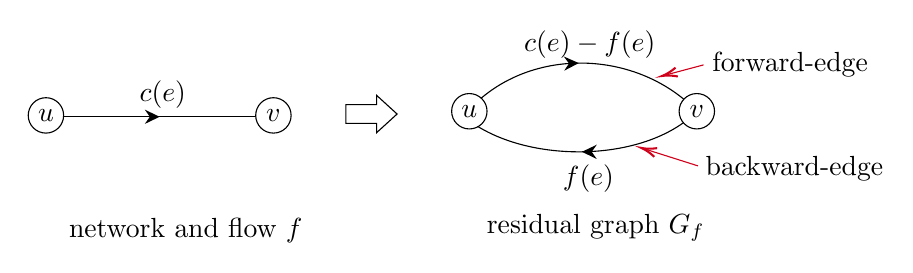
\begin{tikzpicture}[x=0.5pt,y=0.5pt,yscale=-1,xscale=1]
%uncomment if require: \path (0,177); %set diagram left start at 0, and has height of 177

%Curve Lines [id:da27260410535946566] 
\draw    (321,73) .. controls (363,22) and (445,23) .. (489.62,69.5) ;
\draw [shift={(404.33,34.69)}, rotate = 538.0899999999999] [fill={rgb, 255:red, 0; green, 0; blue, 0 }  ][line width=0.08]  [draw opacity=0] (10.72,-5.15) -- (0,0) -- (10.72,5.15) -- (7.12,0) -- cycle    ;
%Curve Lines [id:da29997342467331434] 
\draw    (321,73) .. controls (362,108) and (452,108) .. (489.62,69.5) ;
\draw [shift={(406.58,98.81)}, rotate = 0.2] [fill={rgb, 255:red, 0; green, 0; blue, 0 }  ][line width=0.08]  [draw opacity=0] (10.72,-5.15) -- (0,0) -- (10.72,5.15) -- (7.12,0) -- cycle    ;
%Straight Lines [id:da010972519675235493] 
\draw    (183.62,73.5) -- (19.22,73.5) ;
\draw [shift={(101.42,73.5)}, rotate = 180] [fill={rgb, 255:red, 0; green, 0; blue, 0 }  ][line width=0.08]  [draw opacity=0] (10.72,-5.15) -- (0,0) -- (10.72,5.15) -- (7.12,0) -- cycle    ;
%Shape: Ellipse [id:dp48830544834331435] 
\draw  [fill={rgb, 255:red, 255; green, 255; blue, 255 }  ,fill opacity=1 ] (6.43,72.5) .. controls (6.43,65.44) and (12.15,59.71) .. (19.22,59.71) .. controls (26.28,59.71) and (32.01,65.44) .. (32.01,72.5) .. controls (32.01,79.57) and (26.28,85.29) .. (19.22,85.29) .. controls (12.15,85.29) and (6.43,79.57) .. (6.43,72.5) -- cycle ;
%Shape: Ellipse [id:dp5269749982517756] 
\draw  [fill={rgb, 255:red, 255; green, 255; blue, 255 }  ,fill opacity=1 ] (170.83,72.5) .. controls (170.83,65.44) and (176.56,59.71) .. (183.62,59.71) .. controls (190.69,59.71) and (196.41,65.44) .. (196.41,72.5) .. controls (196.41,79.57) and (190.69,85.29) .. (183.62,85.29) .. controls (176.56,85.29) and (170.83,79.57) .. (170.83,72.5) -- cycle ;
%Shape: Ellipse [id:dp19207664116491352] 
\draw  [fill={rgb, 255:red, 255; green, 255; blue, 255 }  ,fill opacity=1 ] (312.43,69.5) .. controls (312.43,62.44) and (318.15,56.71) .. (325.22,56.71) .. controls (332.28,56.71) and (338.01,62.44) .. (338.01,69.5) .. controls (338.01,76.57) and (332.28,82.29) .. (325.22,82.29) .. controls (318.15,82.29) and (312.43,76.57) .. (312.43,69.5) -- cycle ;
%Shape: Ellipse [id:dp6327110520101094] 
\draw  [fill={rgb, 255:red, 255; green, 255; blue, 255 }  ,fill opacity=1 ] (476.83,69.5) .. controls (476.83,62.44) and (482.56,56.71) .. (489.62,56.71) .. controls (496.69,56.71) and (502.41,62.44) .. (502.41,69.5) .. controls (502.41,76.57) and (496.69,82.29) .. (489.62,82.29) .. controls (482.56,82.29) and (476.83,76.57) .. (476.83,69.5) -- cycle ;
%Right Arrow [id:dp9435587998338902] 
\draw   (236,64.75) -- (258.2,64.75) -- (258.2,58) -- (273,71.5) -- (258.2,85) -- (258.2,78.25) -- (236,78.25) -- cycle ;
%Straight Lines [id:da786288103209363] 
\draw [color={rgb, 255:red, 208; green, 2; blue, 27 }  ,draw opacity=1 ]   (494.5,36) -- (466.43,43.48) ;
\draw [shift={(464.5,44)}, rotate = 345.07] [color={rgb, 255:red, 208; green, 2; blue, 27 }  ,draw opacity=1 ][line width=0.75]    (10.93,-3.29) .. controls (6.95,-1.4) and (3.31,-0.3) .. (0,0) .. controls (3.31,0.3) and (6.95,1.4) .. (10.93,3.29)   ;
%Straight Lines [id:da5256035535625604] 
\draw [color={rgb, 255:red, 208; green, 2; blue, 27 }  ,draw opacity=1 ]   (490.5,109) -- (451.41,96.6) ;
\draw [shift={(449.5,96)}, rotate = 377.59000000000003] [color={rgb, 255:red, 208; green, 2; blue, 27 }  ,draw opacity=1 ][line width=0.75]    (10.93,-3.29) .. controls (6.95,-1.4) and (3.31,-0.3) .. (0,0) .. controls (3.31,0.3) and (6.95,1.4) .. (10.93,3.29)   ;

% Text Node
\draw (183.62,72.5) node   [align=left] {$\displaystyle v$};
% Text Node
\draw (19.22,72.5) node   [align=left] {$\displaystyle u$};
% Text Node
\draw (85,45.5) node [anchor=north west][inner sep=0.75pt]   [align=left] {$\displaystyle c( e)$};
% Text Node
\draw (489.62,69.5) node   [align=left] {$\displaystyle v$};
% Text Node
\draw (325.22,69.5) node   [align=left] {$\displaystyle u$};
% Text Node
\draw (363,9.5) node [anchor=north west][inner sep=0.75pt]   [align=left] {$\displaystyle c( e) -f( e)$};
% Text Node
\draw (391,106.5) node [anchor=north west][inner sep=0.75pt]   [align=left] {$\displaystyle f( e)$};
% Text Node
\draw (34,145) node [anchor=north west][inner sep=0.75pt]   [align=left] {network and flow $\displaystyle f$};
% Text Node
\draw (336,142) node [anchor=north west][inner sep=0.75pt]   [align=left] {residual graph $\displaystyle G_{f}$};
% Text Node
\draw (499,25) node [anchor=north west][inner sep=0.75pt]   [align=left] {forward-edge};
% Text Node
\draw (494,100) node [anchor=north west][inner sep=0.75pt]   [align=left] {backward-edge};


\end{tikzpicture}

}
\caption{Definition of edges and capacities of the residual graph.}
\label{fig:residual-graph}
\end{figure}

Edges in the residual graph with capacity of 0 will be removed. In other words,
we always assume that edges in the residual graph have positive
capacities. Therefore, if an edge $e = (u,v) \in E$ in the network carries a
flow of 0, i.e., $f(e) = 0$, then the residual graph only includes the
corresponding forward-edge $(u, v)$ with capacity $c_f (u, v) = c(e)$; if an
edge $e = (u, v) \in E$  is \emph{saturated}, i.e., $f (e) = c(e)$, then the residual
graph only includes the corresponding backward-edge $(v, u)$ with capacity
$c_f (v, u) = f(e) = c(e)$. See Figure 2.

\begin{figure}[h]
\centering{

\tikzset{every picture/.style={line width=0.75pt}} %set default line width to 0.75pt        

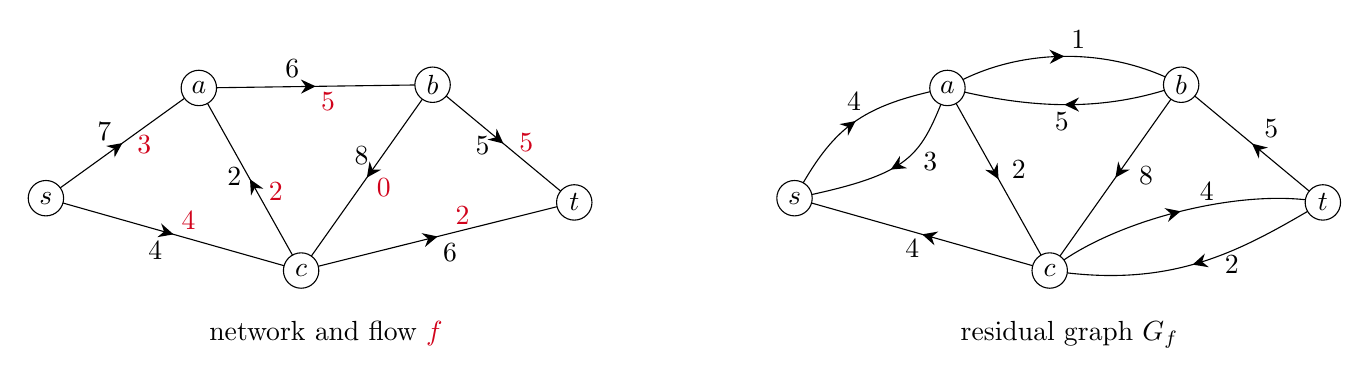
\begin{tikzpicture}[x=0.5pt,y=0.5pt,yscale=-1,xscale=1]
%uncomment if require: \path (0,249); %set diagram left start at 0, and has height of 249

%Curve Lines [id:da5613638706519646] 
\draw    (745.22,183) .. controls (788.5,147) and (885.5,122) .. (942.62,133.78) ;
\draw [shift={(839.83,140.2)}, rotate = 525.5699999999999] [fill={rgb, 255:red, 0; green, 0; blue, 0 }  ][line width=0.08]  [draw opacity=0] (10.72,-5.15) -- (0,0) -- (10.72,5.15) -- (7.12,0) -- cycle    ;
%Curve Lines [id:da2735285843771139] 
\draw    (560.79,130.72) .. controls (588.5,80) and (607.5,64) .. (671.31,51.06) ;
\draw [shift={(604.98,74.96)}, rotate = 503.55] [fill={rgb, 255:red, 0; green, 0; blue, 0 }  ][line width=0.08]  [draw opacity=0] (10.72,-5.15) -- (0,0) -- (10.72,5.15) -- (7.12,0) -- cycle    ;
%Curve Lines [id:da6525683976596537] 
\draw    (671.31,51.06) .. controls (651.5,101) and (647.5,113) .. (560.79,130.72) ;
\draw [shift={(630.35,110.01)}, rotate = 329.68] [fill={rgb, 255:red, 0; green, 0; blue, 0 }  ][line width=0.08]  [draw opacity=0] (10.72,-5.15) -- (0,0) -- (10.72,5.15) -- (7.12,0) -- cycle    ;
%Curve Lines [id:da9916324740026169] 
\draw    (671.31,51.06) .. controls (719.5,22) and (787.5,20) .. (840.22,48.73) ;
\draw [shift={(755.84,28.2)}, rotate = 538.53] [fill={rgb, 255:red, 0; green, 0; blue, 0 }  ][line width=0.08]  [draw opacity=0] (10.72,-5.15) -- (0,0) -- (10.72,5.15) -- (7.12,0) -- cycle    ;
%Curve Lines [id:da8306124055787136] 
\draw    (840.22,48.73) .. controls (789.5,67) and (737.5,68) .. (671.31,51.06) ;
\draw [shift={(755.74,63.12)}, rotate = 359.78] [fill={rgb, 255:red, 0; green, 0; blue, 0 }  ][line width=0.08]  [draw opacity=0] (10.72,-5.15) -- (0,0) -- (10.72,5.15) -- (7.12,0) -- cycle    ;
%Curve Lines [id:da21823822635678936] 
\draw    (942.62,133.78) .. controls (884.5,168) and (835.5,197) .. (745.22,183) ;
\draw [shift={(848.51,178.7)}, rotate = 343.65] [fill={rgb, 255:red, 0; green, 0; blue, 0 }  ][line width=0.08]  [draw opacity=0] (10.72,-5.15) -- (0,0) -- (10.72,5.15) -- (7.12,0) -- cycle    ;
%Straight Lines [id:da06700183790814418] 
\draw    (745.22,183) -- (840.22,48.73) ;
\draw [shift={(792.72,115.86)}, rotate = 305.28] [fill={rgb, 255:red, 0; green, 0; blue, 0 }  ][line width=0.08]  [draw opacity=0] (10.72,-5.15) -- (0,0) -- (10.72,5.15) -- (7.12,0) -- cycle    ;
%Straight Lines [id:da78660649581525] 
\draw    (671.31,51.06) -- (745.22,183) ;
\draw [shift={(708.27,117.03)}, rotate = 240.74] [fill={rgb, 255:red, 0; green, 0; blue, 0 }  ][line width=0.08]  [draw opacity=0] (10.72,-5.15) -- (0,0) -- (10.72,5.15) -- (7.12,0) -- cycle    ;
%Straight Lines [id:da8749205218684325] 
\draw    (745.22,183) -- (560.79,130.72) ;
\draw [shift={(653.01,156.86)}, rotate = 375.83000000000004] [fill={rgb, 255:red, 0; green, 0; blue, 0 }  ][line width=0.08]  [draw opacity=0] (10.72,-5.15) -- (0,0) -- (10.72,5.15) -- (7.12,0) -- cycle    ;
%Straight Lines [id:da4360222788208358] 
\draw    (840.22,48.73) -- (942.62,133.78) ;
\draw [shift={(891.42,91.26)}, rotate = 39.71] [fill={rgb, 255:red, 0; green, 0; blue, 0 }  ][line width=0.08]  [draw opacity=0] (10.72,-5.15) -- (0,0) -- (10.72,5.15) -- (7.12,0) -- cycle    ;
%Shape: Ellipse [id:dp22199319065994672] 
\draw  [fill={rgb, 255:red, 255; green, 255; blue, 255 }  ,fill opacity=1 ] (548,130.72) .. controls (548,123.66) and (553.73,117.93) .. (560.79,117.93) .. controls (567.86,117.93) and (573.58,123.66) .. (573.58,130.72) .. controls (573.58,137.78) and (567.86,143.51) .. (560.79,143.51) .. controls (553.73,143.51) and (548,137.78) .. (548,130.72) -- cycle ;
%Shape: Ellipse [id:dp734016786907147] 
\draw  [fill={rgb, 255:red, 255; green, 255; blue, 255 }  ,fill opacity=1 ] (658.52,51.06) .. controls (658.52,44) and (664.25,38.27) .. (671.31,38.27) .. controls (678.38,38.27) and (684.1,44) .. (684.1,51.06) .. controls (684.1,58.13) and (678.38,63.85) .. (671.31,63.85) .. controls (664.25,63.85) and (658.52,58.13) .. (658.52,51.06) -- cycle ;
%Shape: Ellipse [id:dp6263378369405302] 
\draw  [fill={rgb, 255:red, 255; green, 255; blue, 255 }  ,fill opacity=1 ] (827.43,48.73) .. controls (827.43,41.66) and (833.15,35.94) .. (840.22,35.94) .. controls (847.28,35.94) and (853.01,41.66) .. (853.01,48.73) .. controls (853.01,55.79) and (847.28,61.52) .. (840.22,61.52) .. controls (833.15,61.52) and (827.43,55.79) .. (827.43,48.73) -- cycle ;
%Shape: Ellipse [id:dp7990256965184968] 
\draw  [fill={rgb, 255:red, 255; green, 255; blue, 255 }  ,fill opacity=1 ] (732.43,183) .. controls (732.43,175.94) and (738.15,170.21) .. (745.22,170.21) .. controls (752.28,170.21) and (758.01,175.94) .. (758.01,183) .. controls (758.01,190.06) and (752.28,195.79) .. (745.22,195.79) .. controls (738.15,195.79) and (732.43,190.06) .. (732.43,183) -- cycle ;
%Shape: Ellipse [id:dp7073963568621764] 
\draw  [fill={rgb, 255:red, 255; green, 255; blue, 255 }  ,fill opacity=1 ] (929.83,133.78) .. controls (929.83,126.72) and (935.56,120.99) .. (942.62,120.99) .. controls (949.69,120.99) and (955.41,126.72) .. (955.41,133.78) .. controls (955.41,140.85) and (949.69,146.57) .. (942.62,146.57) .. controls (935.56,146.57) and (929.83,140.85) .. (929.83,133.78) -- cycle ;

%Straight Lines [id:da5195310081734267] 
\draw    (204.22,183) -- (299.22,48.73) ;
\draw [shift={(251.72,115.86)}, rotate = 305.28] [fill={rgb, 255:red, 0; green, 0; blue, 0 }  ][line width=0.08]  [draw opacity=0] (10.72,-5.15) -- (0,0) -- (10.72,5.15) -- (7.12,0) -- cycle    ;
%Straight Lines [id:da4538291997735936] 
\draw    (130.31,51.06) -- (204.22,183) ;
\draw [shift={(167.27,117.03)}, rotate = 60.74] [fill={rgb, 255:red, 0; green, 0; blue, 0 }  ][line width=0.08]  [draw opacity=0] (10.72,-5.15) -- (0,0) -- (10.72,5.15) -- (7.12,0) -- cycle    ;
%Straight Lines [id:da7538382565478482] 
\draw    (19.79,130.72) -- (204.22,183) ;
\draw [shift={(112.01,156.86)}, rotate = 195.83] [fill={rgb, 255:red, 0; green, 0; blue, 0 }  ][line width=0.08]  [draw opacity=0] (10.72,-5.15) -- (0,0) -- (10.72,5.15) -- (7.12,0) -- cycle    ;
%Straight Lines [id:da6748069532380702] 
\draw    (401.62,133.78) -- (204.22,183) ;
\draw [shift={(302.92,158.39)}, rotate = 166] [fill={rgb, 255:red, 0; green, 0; blue, 0 }  ][line width=0.08]  [draw opacity=0] (10.72,-5.15) -- (0,0) -- (10.72,5.15) -- (7.12,0) -- cycle    ;
%Straight Lines [id:da3976427132067899] 
\draw    (19.79,130.72) -- (130.31,51.06) ;
\draw [shift={(75.05,90.89)}, rotate = 504.22] [fill={rgb, 255:red, 0; green, 0; blue, 0 }  ][line width=0.08]  [draw opacity=0] (10.72,-5.15) -- (0,0) -- (10.72,5.15) -- (7.12,0) -- cycle    ;
%Straight Lines [id:da5989756628707282] 
\draw    (299.22,48.73) -- (401.62,133.78) ;
\draw [shift={(350.42,91.26)}, rotate = 219.71] [fill={rgb, 255:red, 0; green, 0; blue, 0 }  ][line width=0.08]  [draw opacity=0] (10.72,-5.15) -- (0,0) -- (10.72,5.15) -- (7.12,0) -- cycle    ;
%Straight Lines [id:da8582315780180115] 
\draw    (130.31,51.06) -- (299.22,48.73) ;
\draw [shift={(214.76,49.89)}, rotate = 539.21] [fill={rgb, 255:red, 0; green, 0; blue, 0 }  ][line width=0.08]  [draw opacity=0] (10.72,-5.15) -- (0,0) -- (10.72,5.15) -- (7.12,0) -- cycle    ;
%Shape: Ellipse [id:dp48011285603633225] 
\draw  [fill={rgb, 255:red, 255; green, 255; blue, 255 }  ,fill opacity=1 ] (7,130.72) .. controls (7,123.66) and (12.73,117.93) .. (19.79,117.93) .. controls (26.86,117.93) and (32.58,123.66) .. (32.58,130.72) .. controls (32.58,137.78) and (26.86,143.51) .. (19.79,143.51) .. controls (12.73,143.51) and (7,137.78) .. (7,130.72) -- cycle ;
%Shape: Ellipse [id:dp34527564053657145] 
\draw  [fill={rgb, 255:red, 255; green, 255; blue, 255 }  ,fill opacity=1 ] (117.52,51.06) .. controls (117.52,44) and (123.25,38.27) .. (130.31,38.27) .. controls (137.38,38.27) and (143.1,44) .. (143.1,51.06) .. controls (143.1,58.13) and (137.38,63.85) .. (130.31,63.85) .. controls (123.25,63.85) and (117.52,58.13) .. (117.52,51.06) -- cycle ;
%Shape: Ellipse [id:dp6239749822676505] 
\draw  [fill={rgb, 255:red, 255; green, 255; blue, 255 }  ,fill opacity=1 ] (286.43,48.73) .. controls (286.43,41.66) and (292.15,35.94) .. (299.22,35.94) .. controls (306.28,35.94) and (312.01,41.66) .. (312.01,48.73) .. controls (312.01,55.79) and (306.28,61.52) .. (299.22,61.52) .. controls (292.15,61.52) and (286.43,55.79) .. (286.43,48.73) -- cycle ;
%Shape: Ellipse [id:dp4869792682336288] 
\draw  [fill={rgb, 255:red, 255; green, 255; blue, 255 }  ,fill opacity=1 ] (191.43,183) .. controls (191.43,175.94) and (197.15,170.21) .. (204.22,170.21) .. controls (211.28,170.21) and (217.01,175.94) .. (217.01,183) .. controls (217.01,190.06) and (211.28,195.79) .. (204.22,195.79) .. controls (197.15,195.79) and (191.43,190.06) .. (191.43,183) -- cycle ;
%Shape: Ellipse [id:dp8101897126294262] 
\draw  [fill={rgb, 255:red, 255; green, 255; blue, 255 }  ,fill opacity=1 ] (388.83,133.78) .. controls (388.83,126.72) and (394.56,120.99) .. (401.62,120.99) .. controls (408.69,120.99) and (414.41,126.72) .. (414.41,133.78) .. controls (414.41,140.85) and (408.69,146.57) .. (401.62,146.57) .. controls (394.56,146.57) and (388.83,140.85) .. (388.83,133.78) -- cycle ;


% Text Node
\draw (136,217.5) node [anchor=north west][inner sep=0.75pt]   [align=left] {network and flow $\displaystyle \textcolor[rgb]{0.82,0.01,0.11}{f}$};
% Text Node
\draw (679,217.5) node [anchor=north west][inner sep=0.75pt]   [align=left] {residual graph $\displaystyle G_{f}$};
% Text Node
\draw (19.79,130.72) node   [align=left] {$\displaystyle s$};
% Text Node
\draw (130.31,51.06) node   [align=left] {$\displaystyle a$};
% Text Node
\draw (299.22,48.73) node   [align=left] {$\displaystyle b$};
% Text Node
\draw (204.22,183) node   [align=left] {$\displaystyle c$};
% Text Node
\draw (401.62,133.78) node   [align=left] {$\displaystyle t$};
% Text Node
\draw (92,159.89) node [anchor=north west][inner sep=0.75pt]   [align=left] {$\displaystyle 4$};
% Text Node
\draw (241,91.89) node [anchor=north west][inner sep=0.75pt]   [align=left] {$\displaystyle 8$};
% Text Node
\draw (149,106.89) node [anchor=north west][inner sep=0.75pt]   [align=left] {$\displaystyle 2$};
% Text Node
\draw (55,73.89) node [anchor=north west][inner sep=0.75pt]   [align=left] {$\displaystyle 7$};
% Text Node
\draw (304.92,161.39) node [anchor=north west][inner sep=0.75pt]   [align=left] {$\displaystyle 6$};
% Text Node
\draw (328.42,84.26) node [anchor=north west][inner sep=0.75pt]   [align=left] {$\displaystyle 5$};
% Text Node
\draw (191,28.89) node [anchor=north west][inner sep=0.75pt]   [align=left] {$\displaystyle 6$};
% Text Node
\draw (116,138.89) node [anchor=north west][inner sep=0.75pt]   [align=left] {$\displaystyle \textcolor[rgb]{0.82,0.01,0.11}{4}$};
% Text Node
\draw (179,117.89) node [anchor=north west][inner sep=0.75pt]   [align=left] {$\displaystyle \textcolor[rgb]{0.82,0.01,0.11}{2}$};
% Text Node
\draw (314,134.89) node [anchor=north west][inner sep=0.75pt]   [align=left] {$\displaystyle \textcolor[rgb]{0.82,0.01,0.11}{2}$};
% Text Node
\draw (84,83.89) node [anchor=north west][inner sep=0.75pt]   [align=left] {$\displaystyle \textcolor[rgb]{0.82,0.01,0.11}{3}$};
% Text Node
\draw (216.76,52.89) node [anchor=north west][inner sep=0.75pt]   [align=left] {$\displaystyle \textcolor[rgb]{0.82,0.01,0.11}{5}$};
% Text Node
\draw (257,114.89) node [anchor=north west][inner sep=0.75pt]   [align=left] {$\displaystyle \textcolor[rgb]{0.82,0.01,0.11}{0}$};
% Text Node
\draw (360,81.89) node [anchor=north west][inner sep=0.75pt]   [align=left] {$\displaystyle \textcolor[rgb]{0.82,0.01,0.11}{5}$};
% Text Node
\draw (560.79,130.72) node   [align=left] {$\displaystyle s$};
% Text Node
\draw (671.31,51.06) node   [align=left] {$\displaystyle a$};
% Text Node
\draw (840.22,48.73) node   [align=left] {$\displaystyle b$};
% Text Node
\draw (745.22,183) node   [align=left] {$\displaystyle c$};
% Text Node
\draw (942.62,133.78) node   [align=left] {$\displaystyle t$};
% Text Node
\draw (652,95.89) node [anchor=north west][inner sep=0.75pt]   [align=left] {$\displaystyle 3$};
% Text Node
\draw (808,105.89) node [anchor=north west][inner sep=0.75pt]   [align=left] {$\displaystyle 8$};
% Text Node
\draw (716,101.89) node [anchor=north west][inner sep=0.75pt]   [align=left] {$\displaystyle 2$};
% Text Node
\draw (597,52.89) node [anchor=north west][inner sep=0.75pt]   [align=left] {$\displaystyle 4$};
% Text Node
\draw (851.92,117.39) node [anchor=north west][inner sep=0.75pt]   [align=left] {$\displaystyle 4$};
% Text Node
\draw (898.42,72.26) node [anchor=north west][inner sep=0.75pt]   [align=left] {$\displaystyle 5$};
% Text Node
\draw (759,7.89) node [anchor=north west][inner sep=0.75pt]   [align=left] {$\displaystyle 1$};
% Text Node
\draw (639,158.89) node [anchor=north west][inner sep=0.75pt]   [align=left] {$\displaystyle 4$};
% Text Node
\draw (747,66.89) node [anchor=north west][inner sep=0.75pt]   [align=left] {$\displaystyle 5$};
% Text Node
\draw (869.92,170.39) node [anchor=north west][inner sep=0.75pt]   [align=left] {$\displaystyle 2$};


\end{tikzpicture}

}
\caption{An example of residual graph.}
\label{fig:example}
\end{figure}

%\subsection*{The Ford-Fulkson Algorithm}

{\bf Finding an $s$-$t$ path in $G_f$.}
%Recall that the central idea of the FF algorithm is to iteratively improve an $s$-$t$ flow $f$, initialized with $f(e) = 0$ for every $e \in E$. 
In each iteration of the Ford-Fulkson algorithm, after building $G_f$ wrt the current flow $f$,
it seeks a path $p$ from $s$ to $t$, called an $s$-$t$ path, in residual graph $G_f$.
The searching of such $s$-$t$ path can be done by either BFS or DFS, starting from $s$.
If such path cannot be found, the algorithm terminates and returns the current flow $f$.
Otherwise, it \emph{augments} $p$ to obtain a flow with increased value. 

{\bf Augmenting an $s$-$t$ path $p$ in $G_f$.}
To augment an $s$-$t$ path $p$ in $G_f$, we first calcualte the bottleneck capacity of
$p$, which is defined as the smallest capacity~(in the residual graph $G_f$) of all edges in $p$, formally
written as $x(p) := \min_{e\in p} c_f(e)$. We then examine each edge $e \in p$, and
update the flow of the corresponding edge in the network with the following rule.

\vspace*{-\topsep}
\begin{enumerate}
\item If $e = (u,v) \in p$ is a forward edge, i.e., $(u,v)$ is in the network, we update $f(u,v) \leftarrow f(u,v)+x(p)$;
\item If $e = (u,v) \in p$ is a backward edge, i.e., $(v,u)$ is in the network, we update $f(v,u) \leftarrow f(v,u)-x(p)$;
\end{enumerate}

The flow of other edges in the network (i.e., none of their corresponding
forward edges or backward edges is in $p$) will not get affected. See an
example in Figure~\ref{fig:augment}.

\begin{figure}[h]
\centering{

\tikzset{every picture/.style={line width=0.75pt}} %set default line width to 0.75pt        

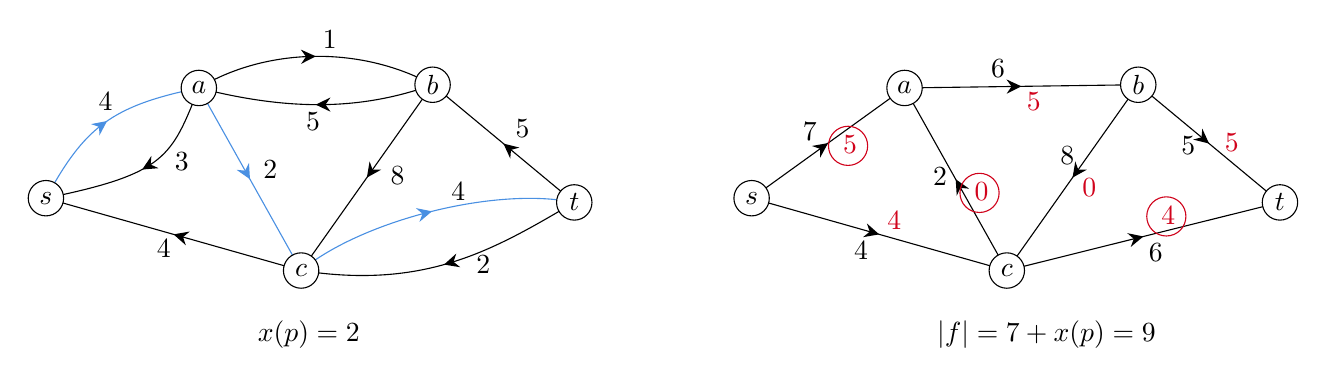
\begin{tikzpicture}[x=0.5pt,y=0.5pt,yscale=-1,xscale=1]
%uncomment if require: \path (0,252); %set diagram left start at 0, and has height of 252

%Curve Lines [id:da5613638706519646] 
\draw [color={rgb, 255:red, 74; green, 144; blue, 226 }  ,draw opacity=1 ]   (202.22,187) .. controls (245.5,151) and (342.5,126) .. (399.62,137.78) ;
\draw [shift={(296.83,144.2)}, rotate = 525.5699999999999] [fill={rgb, 255:red, 74; green, 144; blue, 226 }  ,fill opacity=1 ][line width=0.08]  [draw opacity=0] (10.72,-5.15) -- (0,0) -- (10.72,5.15) -- (7.12,0) -- cycle    ;
%Curve Lines [id:da2735285843771139] 
\draw [color={rgb, 255:red, 74; green, 144; blue, 226 }  ,draw opacity=1 ]   (17.79,134.72) .. controls (45.5,84) and (64.5,68) .. (128.31,55.06) ;
\draw [shift={(61.98,78.96)}, rotate = 503.55] [fill={rgb, 255:red, 74; green, 144; blue, 226 }  ,fill opacity=1 ][line width=0.08]  [draw opacity=0] (10.72,-5.15) -- (0,0) -- (10.72,5.15) -- (7.12,0) -- cycle    ;
%Curve Lines [id:da6525683976596537] 
\draw    (128.31,55.06) .. controls (108.5,105) and (104.5,117) .. (17.79,134.72) ;
\draw [shift={(87.35,114.01)}, rotate = 329.68] [fill={rgb, 255:red, 0; green, 0; blue, 0 }  ][line width=0.08]  [draw opacity=0] (10.72,-5.15) -- (0,0) -- (10.72,5.15) -- (7.12,0) -- cycle    ;
%Curve Lines [id:da9916324740026169] 
\draw    (128.31,55.06) .. controls (176.5,26) and (244.5,24) .. (297.22,52.73) ;
\draw [shift={(212.84,32.2)}, rotate = 538.53] [fill={rgb, 255:red, 0; green, 0; blue, 0 }  ][line width=0.08]  [draw opacity=0] (10.72,-5.15) -- (0,0) -- (10.72,5.15) -- (7.12,0) -- cycle    ;
%Curve Lines [id:da8306124055787136] 
\draw    (297.22,52.73) .. controls (246.5,71) and (194.5,72) .. (128.31,55.06) ;
\draw [shift={(212.74,67.12)}, rotate = 359.78] [fill={rgb, 255:red, 0; green, 0; blue, 0 }  ][line width=0.08]  [draw opacity=0] (10.72,-5.15) -- (0,0) -- (10.72,5.15) -- (7.12,0) -- cycle    ;
%Curve Lines [id:da21823822635678936] 
\draw    (399.62,137.78) .. controls (341.5,172) and (292.5,201) .. (202.22,187) ;
\draw [shift={(305.51,182.7)}, rotate = 343.65] [fill={rgb, 255:red, 0; green, 0; blue, 0 }  ][line width=0.08]  [draw opacity=0] (10.72,-5.15) -- (0,0) -- (10.72,5.15) -- (7.12,0) -- cycle    ;
%Straight Lines [id:da06700183790814418] 
\draw    (202.22,187) -- (297.22,52.73) ;
\draw [shift={(249.72,119.86)}, rotate = 305.28] [fill={rgb, 255:red, 0; green, 0; blue, 0 }  ][line width=0.08]  [draw opacity=0] (10.72,-5.15) -- (0,0) -- (10.72,5.15) -- (7.12,0) -- cycle    ;
%Straight Lines [id:da78660649581525] 
\draw [color={rgb, 255:red, 74; green, 144; blue, 226 }  ,draw opacity=1 ]   (128.31,55.06) -- (202.22,187) ;
\draw [shift={(165.27,121.03)}, rotate = 240.74] [fill={rgb, 255:red, 74; green, 144; blue, 226 }  ,fill opacity=1 ][line width=0.08]  [draw opacity=0] (10.72,-5.15) -- (0,0) -- (10.72,5.15) -- (7.12,0) -- cycle    ;
%Straight Lines [id:da8749205218684325] 
\draw    (202.22,187) -- (17.79,134.72) ;
\draw [shift={(110.01,160.86)}, rotate = 375.83000000000004] [fill={rgb, 255:red, 0; green, 0; blue, 0 }  ][line width=0.08]  [draw opacity=0] (10.72,-5.15) -- (0,0) -- (10.72,5.15) -- (7.12,0) -- cycle    ;
%Straight Lines [id:da4360222788208358] 
\draw    (297.22,52.73) -- (399.62,137.78) ;
\draw [shift={(348.42,95.26)}, rotate = 39.71] [fill={rgb, 255:red, 0; green, 0; blue, 0 }  ][line width=0.08]  [draw opacity=0] (10.72,-5.15) -- (0,0) -- (10.72,5.15) -- (7.12,0) -- cycle    ;
%Shape: Ellipse [id:dp22199319065994672] 
\draw  [fill={rgb, 255:red, 255; green, 255; blue, 255 }  ,fill opacity=1 ] (5,134.72) .. controls (5,127.66) and (10.73,121.93) .. (17.79,121.93) .. controls (24.86,121.93) and (30.58,127.66) .. (30.58,134.72) .. controls (30.58,141.78) and (24.86,147.51) .. (17.79,147.51) .. controls (10.73,147.51) and (5,141.78) .. (5,134.72) -- cycle ;
%Shape: Ellipse [id:dp734016786907147] 
\draw  [fill={rgb, 255:red, 255; green, 255; blue, 255 }  ,fill opacity=1 ] (115.52,55.06) .. controls (115.52,48) and (121.25,42.27) .. (128.31,42.27) .. controls (135.38,42.27) and (141.1,48) .. (141.1,55.06) .. controls (141.1,62.13) and (135.38,67.85) .. (128.31,67.85) .. controls (121.25,67.85) and (115.52,62.13) .. (115.52,55.06) -- cycle ;
%Shape: Ellipse [id:dp6263378369405302] 
\draw  [fill={rgb, 255:red, 255; green, 255; blue, 255 }  ,fill opacity=1 ] (284.43,52.73) .. controls (284.43,45.66) and (290.15,39.94) .. (297.22,39.94) .. controls (304.28,39.94) and (310.01,45.66) .. (310.01,52.73) .. controls (310.01,59.79) and (304.28,65.52) .. (297.22,65.52) .. controls (290.15,65.52) and (284.43,59.79) .. (284.43,52.73) -- cycle ;
%Shape: Ellipse [id:dp7990256965184968] 
\draw  [fill={rgb, 255:red, 255; green, 255; blue, 255 }  ,fill opacity=1 ] (189.43,187) .. controls (189.43,179.94) and (195.15,174.21) .. (202.22,174.21) .. controls (209.28,174.21) and (215.01,179.94) .. (215.01,187) .. controls (215.01,194.06) and (209.28,199.79) .. (202.22,199.79) .. controls (195.15,199.79) and (189.43,194.06) .. (189.43,187) -- cycle ;
%Shape: Ellipse [id:dp7073963568621764] 
\draw  [fill={rgb, 255:red, 255; green, 255; blue, 255 }  ,fill opacity=1 ] (386.83,137.78) .. controls (386.83,130.72) and (392.56,124.99) .. (399.62,124.99) .. controls (406.69,124.99) and (412.41,130.72) .. (412.41,137.78) .. controls (412.41,144.85) and (406.69,150.57) .. (399.62,150.57) .. controls (392.56,150.57) and (386.83,144.85) .. (386.83,137.78) -- cycle ;
%Straight Lines [id:da5195310081734267] 
\draw    (712.22,187) -- (807.22,52.73) ;
\draw [shift={(759.72,119.86)}, rotate = 305.28] [fill={rgb, 255:red, 0; green, 0; blue, 0 }  ][line width=0.08]  [draw opacity=0] (10.72,-5.15) -- (0,0) -- (10.72,5.15) -- (7.12,0) -- cycle    ;
%Straight Lines [id:da4538291997735936] 
\draw    (638.31,55.06) -- (712.22,187) ;
\draw [shift={(675.27,121.03)}, rotate = 60.74] [fill={rgb, 255:red, 0; green, 0; blue, 0 }  ][line width=0.08]  [draw opacity=0] (10.72,-5.15) -- (0,0) -- (10.72,5.15) -- (7.12,0) -- cycle    ;
%Straight Lines [id:da7538382565478482] 
\draw    (527.79,134.72) -- (712.22,187) ;
\draw [shift={(620.01,160.86)}, rotate = 195.83] [fill={rgb, 255:red, 0; green, 0; blue, 0 }  ][line width=0.08]  [draw opacity=0] (10.72,-5.15) -- (0,0) -- (10.72,5.15) -- (7.12,0) -- cycle    ;
%Straight Lines [id:da6748069532380702] 
\draw    (909.62,137.78) -- (712.22,187) ;
\draw [shift={(810.92,162.39)}, rotate = 166] [fill={rgb, 255:red, 0; green, 0; blue, 0 }  ][line width=0.08]  [draw opacity=0] (10.72,-5.15) -- (0,0) -- (10.72,5.15) -- (7.12,0) -- cycle    ;
%Straight Lines [id:da3976427132067899] 
\draw    (527.79,134.72) -- (638.31,55.06) ;
\draw [shift={(583.05,94.89)}, rotate = 504.22] [fill={rgb, 255:red, 0; green, 0; blue, 0 }  ][line width=0.08]  [draw opacity=0] (10.72,-5.15) -- (0,0) -- (10.72,5.15) -- (7.12,0) -- cycle    ;
%Straight Lines [id:da5989756628707282] 
\draw    (807.22,52.73) -- (909.62,137.78) ;
\draw [shift={(858.42,95.26)}, rotate = 219.71] [fill={rgb, 255:red, 0; green, 0; blue, 0 }  ][line width=0.08]  [draw opacity=0] (10.72,-5.15) -- (0,0) -- (10.72,5.15) -- (7.12,0) -- cycle    ;
%Straight Lines [id:da8582315780180115] 
\draw    (638.31,55.06) -- (807.22,52.73) ;
\draw [shift={(722.76,53.89)}, rotate = 539.21] [fill={rgb, 255:red, 0; green, 0; blue, 0 }  ][line width=0.08]  [draw opacity=0] (10.72,-5.15) -- (0,0) -- (10.72,5.15) -- (7.12,0) -- cycle    ;
%Shape: Ellipse [id:dp48011285603633225] 
\draw  [fill={rgb, 255:red, 255; green, 255; blue, 255 }  ,fill opacity=1 ] (515,134.72) .. controls (515,127.66) and (520.73,121.93) .. (527.79,121.93) .. controls (534.86,121.93) and (540.58,127.66) .. (540.58,134.72) .. controls (540.58,141.78) and (534.86,147.51) .. (527.79,147.51) .. controls (520.73,147.51) and (515,141.78) .. (515,134.72) -- cycle ;
%Shape: Ellipse [id:dp34527564053657145] 
\draw  [fill={rgb, 255:red, 255; green, 255; blue, 255 }  ,fill opacity=1 ] (625.52,55.06) .. controls (625.52,48) and (631.25,42.27) .. (638.31,42.27) .. controls (645.38,42.27) and (651.1,48) .. (651.1,55.06) .. controls (651.1,62.13) and (645.38,67.85) .. (638.31,67.85) .. controls (631.25,67.85) and (625.52,62.13) .. (625.52,55.06) -- cycle ;
%Shape: Ellipse [id:dp6239749822676505] 
\draw  [fill={rgb, 255:red, 255; green, 255; blue, 255 }  ,fill opacity=1 ] (794.43,52.73) .. controls (794.43,45.66) and (800.15,39.94) .. (807.22,39.94) .. controls (814.28,39.94) and (820.01,45.66) .. (820.01,52.73) .. controls (820.01,59.79) and (814.28,65.52) .. (807.22,65.52) .. controls (800.15,65.52) and (794.43,59.79) .. (794.43,52.73) -- cycle ;
%Shape: Ellipse [id:dp4869792682336288] 
\draw  [fill={rgb, 255:red, 255; green, 255; blue, 255 }  ,fill opacity=1 ] (699.43,187) .. controls (699.43,179.94) and (705.15,174.21) .. (712.22,174.21) .. controls (719.28,174.21) and (725.01,179.94) .. (725.01,187) .. controls (725.01,194.06) and (719.28,199.79) .. (712.22,199.79) .. controls (705.15,199.79) and (699.43,194.06) .. (699.43,187) -- cycle ;
%Shape: Ellipse [id:dp8101897126294262] 
\draw  [fill={rgb, 255:red, 255; green, 255; blue, 255 }  ,fill opacity=1 ] (896.83,137.78) .. controls (896.83,130.72) and (902.56,124.99) .. (909.62,124.99) .. controls (916.69,124.99) and (922.41,130.72) .. (922.41,137.78) .. controls (922.41,144.85) and (916.69,150.57) .. (909.62,150.57) .. controls (902.56,150.57) and (896.83,144.85) .. (896.83,137.78) -- cycle ;

% Text Node
\draw (527.79,134.72) node   [align=left] {$\displaystyle s$};
% Text Node
\draw (638.31,55.06) node   [align=left] {$\displaystyle a$};
% Text Node
\draw (807.22,52.73) node   [align=left] {$\displaystyle b$};
% Text Node
\draw (712.22,187) node   [align=left] {$\displaystyle c$};
% Text Node
\draw (909.62,137.78) node   [align=left] {$\displaystyle t$};
% Text Node
\draw (600,163.89) node [anchor=north west][inner sep=0.75pt]   [align=left] {$\displaystyle 4$};
% Text Node
\draw (749,95.89) node [anchor=north west][inner sep=0.75pt]   [align=left] {$\displaystyle 8$};
% Text Node
\draw (657,110.89) node [anchor=north west][inner sep=0.75pt]   [align=left] {$\displaystyle 2$};
% Text Node
\draw (563,77.89) node [anchor=north west][inner sep=0.75pt]   [align=left] {$\displaystyle 7$};
% Text Node
\draw (812.92,165.39) node [anchor=north west][inner sep=0.75pt]   [align=left] {$\displaystyle 6$};
% Text Node
\draw (836.42,88.26) node [anchor=north west][inner sep=0.75pt]   [align=left] {$\displaystyle 5$};
% Text Node
\draw (699,32.89) node [anchor=north west][inner sep=0.75pt]   [align=left] {$\displaystyle 6$};
% Text Node
\draw (624,142.89) node [anchor=north west][inner sep=0.75pt]   [align=left] {$\displaystyle \textcolor[rgb]{0.82,0.01,0.11}{4}$};
% Text Node
\draw  [color={rgb, 255:red, 208; green, 2; blue, 27 }  ,draw opacity=1 ]  (692.5, 130.89) circle [x radius= 14.15, y radius= 14.15]   ;
\draw (687,121.89) node [anchor=north west][inner sep=0.75pt]   [align=left] {$\displaystyle \textcolor[rgb]{0.82,0.01,0.11}{0}$};
% Text Node
\draw  [color={rgb, 255:red, 208; green, 2; blue, 27 }  ,draw opacity=1 ]  (827.5, 147.89) circle [x radius= 14.15, y radius= 14.15]   ;
\draw (822,138.89) node [anchor=north west][inner sep=0.75pt]   [align=left] {$\displaystyle \textcolor[rgb]{0.82,0.01,0.11}{4}$};
% Text Node
\draw  [color={rgb, 255:red, 208; green, 2; blue, 27 }  ,draw opacity=1 ]  (597.5, 96.89) circle [x radius= 14.15, y radius= 14.15]   ;
\draw (592,87.89) node [anchor=north west][inner sep=0.75pt]   [align=left] {$\displaystyle \textcolor[rgb]{0.82,0.01,0.11}{5}$};
% Text Node
\draw (724.76,56.89) node [anchor=north west][inner sep=0.75pt]   [align=left] {$\displaystyle \textcolor[rgb]{0.82,0.01,0.11}{5}$};
% Text Node
\draw (765,118.89) node [anchor=north west][inner sep=0.75pt]   [align=left] {$\displaystyle \textcolor[rgb]{0.82,0.01,0.11}{0}$};
% Text Node
\draw (868,85.89) node [anchor=north west][inner sep=0.75pt]   [align=left] {$\displaystyle \textcolor[rgb]{0.82,0.01,0.11}{5}$};
% Text Node
\draw (17.79,134.72) node   [align=left] {$\displaystyle s$};
% Text Node
\draw (128.31,55.06) node   [align=left] {$\displaystyle a$};
% Text Node
\draw (297.22,52.73) node   [align=left] {$\displaystyle b$};
% Text Node
\draw (202.22,187) node   [align=left] {$\displaystyle c$};
% Text Node
\draw (399.62,137.78) node   [align=left] {$\displaystyle t$};
% Text Node
\draw (109,99.89) node [anchor=north west][inner sep=0.75pt]   [align=left] {$\displaystyle 3$};
% Text Node
\draw (265,109.89) node [anchor=north west][inner sep=0.75pt]   [align=left] {$\displaystyle 8$};
% Text Node
\draw (173,105.89) node [anchor=north west][inner sep=0.75pt]   [align=left] {$\displaystyle 2$};
% Text Node
\draw (54,56.89) node [anchor=north west][inner sep=0.75pt]   [align=left] {$\displaystyle 4$};
% Text Node
\draw (308.92,121.39) node [anchor=north west][inner sep=0.75pt]   [align=left] {$\displaystyle 4$};
% Text Node
\draw (355.42,76.26) node [anchor=north west][inner sep=0.75pt]   [align=left] {$\displaystyle 5$};
% Text Node
\draw (216,11.89) node [anchor=north west][inner sep=0.75pt]   [align=left] {$\displaystyle 1$};
% Text Node
\draw (96,162.89) node [anchor=north west][inner sep=0.75pt]   [align=left] {$\displaystyle 4$};
% Text Node
\draw (204,70.89) node [anchor=north west][inner sep=0.75pt]   [align=left] {$\displaystyle 5$};
% Text Node
\draw (326.92,174.39) node [anchor=north west][inner sep=0.75pt]   [align=left] {$\displaystyle 2$};
% Text Node
\draw (169,221.5) node [anchor=north west][inner sep=0.75pt]   [align=left] {$\displaystyle x( p) =2$};
% Text Node
\draw (660,221.5) node [anchor=north west][inner sep=0.75pt]   [align=left] {$\displaystyle |f|=7+x( p) =9$};


\end{tikzpicture}

}
\caption{Illustrating the procedure of augmenting continuing Figure~\ref{fig:example}. Suppose
in the residual graph $G_f$ given in Figure~\ref{fig:example} the algorithm identifies $s$-$t$
path $p = (s,a,c,t)$. Note that in this path $(s,a)$ and $(c,t)$ are forward
edges and $(a, c)$ is backward edge. After augmenting $p$ the flow $f$ is given in the right figure,
where affected flow are circled.}
\label{fig:augment}
\end{figure}

We emphasize that, after augmenting, $f$ remains a valid flow, i.e., $f$ satisfies
both the capacity condition and the conservation condition. The capacity
condition remains satisfied owes to how the residual graph is constructed.
Consider the two cases in augmenting: in either case, after augmenting, the
flow remains non-negative and bounded by the capacity. Specifically,

\vspace*{-\topsep}
\begin{enumerate}
\item if $e=(u,v)\in p$ is a forward edge, we know that $c_f(e)=c(u,v)-f(u,v)$ based on the
construction of the residual graph. Since $x( p) \le c_f (e)$, after augmenting the
flow of edge $(u, v)$ becomes $f(u, v) + x(p) \le f(u,v)+c_f (e) = f(u,v)+c(u,v)- f(u,v) = c(u,v)$. 
And it’s obvious that $f(u,v)+x(p) \ge 0$.
\item if $e=(u,v)\in p$ is a backward edge, we know that $c_f(e)=f(v,u)$ based on the
construction of the residual graph. Since $x(p) \le c_f(e)$, after augmenting the
flow of edge $(v, u)$ becomes $f(v, u) - x(p) \ge f(v,u)-c_f (e) = f(v,u)-f(v,u) = 0$. 
And it’s obvious that $f(v,u)-x(p) \le f(v,u) \le c(v,u)$.
\end{enumerate}

\begin{figure}[!b]
\centering{

\tikzset{every picture/.style={line width=0.75pt}} %set default line width to 0.75pt        

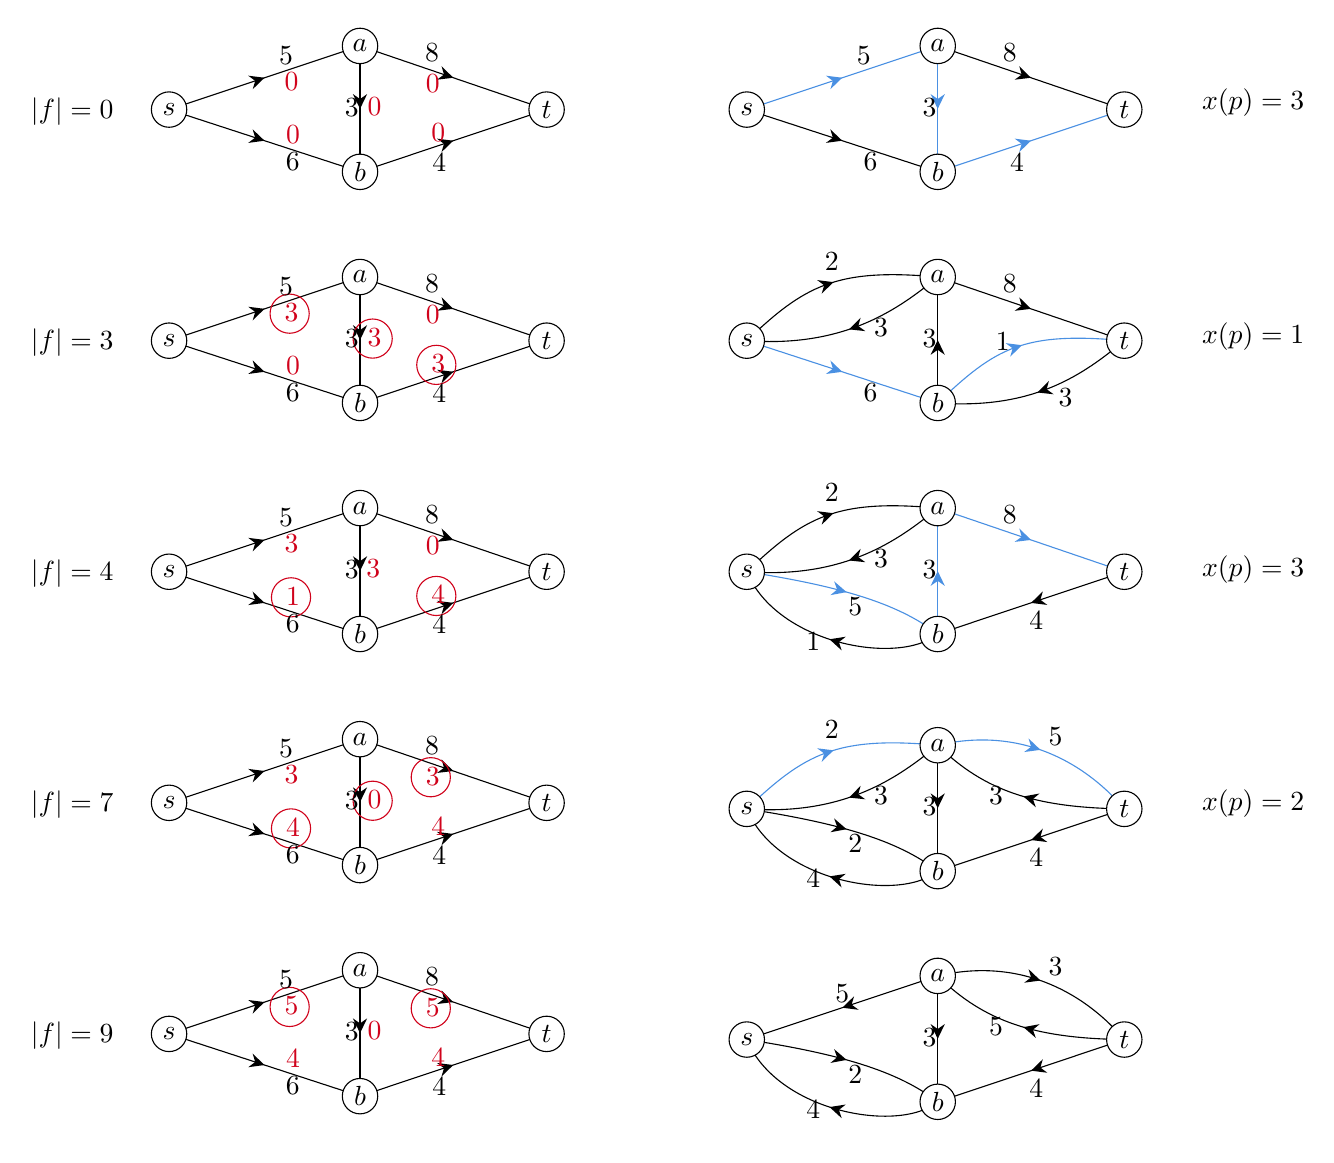
\begin{tikzpicture}[x=0.5pt,y=0.5pt,yscale=-1,xscale=1]
%uncomment if require: \path (0,839); %set diagram left start at 0, and has height of 839

%Straight Lines [id:da5712618432248621] 
\draw    (824.12,415.76) -- (689.29,460.76) ;
\draw [shift={(756.71,438.26)}, rotate = 341.53999999999996] [fill={rgb, 255:red, 0; green, 0; blue, 0 }  ][line width=0.08]  [draw opacity=0] (10.72,-5.15) -- (0,0) -- (10.72,5.15) -- (7.12,0) -- cycle    ;
%Curve Lines [id:da21939430850053032] 
\draw [color={rgb, 255:red, 74; green, 144; blue, 226 }  ,draw opacity=1 ]   (551.29,415.76) .. controls (617,426.01) and (660,438.01) .. (689.29,460.76) ;
\draw [shift={(623.46,430.47)}, rotate = 195.08] [fill={rgb, 255:red, 74; green, 144; blue, 226 }  ,fill opacity=1 ][line width=0.08]  [draw opacity=0] (10.72,-5.15) -- (0,0) -- (10.72,5.15) -- (7.12,0) -- cycle    ;
%Curve Lines [id:da15773096786649754] 
\draw    (689.29,460.76) .. controls (661,484.01) and (573,468.01) .. (551.29,415.76) ;
\draw [shift={(611.07,464.56)}, rotate = 376.76] [fill={rgb, 255:red, 0; green, 0; blue, 0 }  ][line width=0.08]  [draw opacity=0] (10.72,-5.15) -- (0,0) -- (10.72,5.15) -- (7.12,0) -- cycle    ;
%Straight Lines [id:da024680351236297304] 
\draw [color={rgb, 255:red, 74; green, 144; blue, 226 }  ,draw opacity=1 ]   (689.29,369.76) -- (824.12,415.76) ;
\draw [shift={(756.71,392.76)}, rotate = 198.84] [fill={rgb, 255:red, 74; green, 144; blue, 226 }  ,fill opacity=1 ][line width=0.08]  [draw opacity=0] (10.72,-5.15) -- (0,0) -- (10.72,5.15) -- (7.12,0) -- cycle    ;
%Curve Lines [id:da14623738071334857] 
\draw    (551.29,415.76) .. controls (593,376.01) and (616,363.01) .. (689.29,369.76) ;
\draw [shift={(613.98,373.47)}, rotate = 521.52] [fill={rgb, 255:red, 0; green, 0; blue, 0 }  ][line width=0.08]  [draw opacity=0] (10.72,-5.15) -- (0,0) -- (10.72,5.15) -- (7.12,0) -- cycle    ;
%Curve Lines [id:da1884084092202849] 
\draw    (689.29,369.76) .. controls (661,393.01) and (622,421.01) .. (551.29,415.76) ;
\draw [shift={(625.16,407.6)}, rotate = 340.45] [fill={rgb, 255:red, 0; green, 0; blue, 0 }  ][line width=0.08]  [draw opacity=0] (10.72,-5.15) -- (0,0) -- (10.72,5.15) -- (7.12,0) -- cycle    ;
%Straight Lines [id:da5031539886046075] 
\draw [color={rgb, 255:red, 74; green, 144; blue, 226 }  ,draw opacity=1 ]   (689.29,369.76) -- (689.29,460.76) ;
\draw [shift={(689.29,415.26)}, rotate = 90] [fill={rgb, 255:red, 74; green, 144; blue, 226 }  ,fill opacity=1 ][line width=0.08]  [draw opacity=0] (10.72,-5.15) -- (0,0) -- (10.72,5.15) -- (7.12,0) -- cycle    ;
%Shape: Ellipse [id:dp5508071293563598] 
\draw  [fill={rgb, 255:red, 255; green, 255; blue, 255 }  ,fill opacity=1 ] (538.5,415.76) .. controls (538.5,408.7) and (544.23,402.97) .. (551.29,402.97) .. controls (558.36,402.97) and (564.08,408.7) .. (564.08,415.76) .. controls (564.08,422.83) and (558.36,428.55) .. (551.29,428.55) .. controls (544.23,428.55) and (538.5,422.83) .. (538.5,415.76) -- cycle ;
%Shape: Ellipse [id:dp5972831071444443] 
\draw  [fill={rgb, 255:red, 255; green, 255; blue, 255 }  ,fill opacity=1 ] (811.33,415.76) .. controls (811.33,408.7) and (817.06,402.97) .. (824.12,402.97) .. controls (831.19,402.97) and (836.91,408.7) .. (836.91,415.76) .. controls (836.91,422.83) and (831.19,428.55) .. (824.12,428.55) .. controls (817.06,428.55) and (811.33,422.83) .. (811.33,415.76) -- cycle ;
%Shape: Ellipse [id:dp04179037888015247] 
\draw  [fill={rgb, 255:red, 255; green, 255; blue, 255 }  ,fill opacity=1 ] (676.5,369.76) .. controls (676.5,362.7) and (682.23,356.97) .. (689.29,356.97) .. controls (696.36,356.97) and (702.08,362.7) .. (702.08,369.76) .. controls (702.08,376.83) and (696.36,382.55) .. (689.29,382.55) .. controls (682.23,382.55) and (676.5,376.83) .. (676.5,369.76) -- cycle ;
%Shape: Ellipse [id:dp6412358417638034] 
\draw  [fill={rgb, 255:red, 255; green, 255; blue, 255 }  ,fill opacity=1 ] (676.5,460.76) .. controls (676.5,453.7) and (682.23,447.97) .. (689.29,447.97) .. controls (696.36,447.97) and (702.08,453.7) .. (702.08,460.76) .. controls (702.08,467.83) and (696.36,473.55) .. (689.29,473.55) .. controls (682.23,473.55) and (676.5,467.83) .. (676.5,460.76) -- cycle ;

%Straight Lines [id:da7930208884666833] 
\draw    (824.12,587.12) -- (689.29,632.12) ;
\draw [shift={(756.71,609.62)}, rotate = 341.53999999999996] [fill={rgb, 255:red, 0; green, 0; blue, 0 }  ][line width=0.08]  [draw opacity=0] (10.72,-5.15) -- (0,0) -- (10.72,5.15) -- (7.12,0) -- cycle    ;
%Curve Lines [id:da7926875310432893] 
\draw [color={rgb, 255:red, 74; green, 144; blue, 226 }  ,draw opacity=1 ]   (689.29,541.12) .. controls (753,526.36) and (799,557.36) .. (824.12,587.12) ;
\draw [shift={(763.54,544.46)}, rotate = 198.02] [fill={rgb, 255:red, 74; green, 144; blue, 226 }  ,fill opacity=1 ][line width=0.08]  [draw opacity=0] (10.72,-5.15) -- (0,0) -- (10.72,5.15) -- (7.12,0) -- cycle    ;
%Curve Lines [id:da34610507417952074] 
\draw    (824.12,587.12) .. controls (760,586.36) and (723,574.36) .. (689.29,541.12) ;
\draw [shift={(751.2,578.16)}, rotate = 375.31] [fill={rgb, 255:red, 0; green, 0; blue, 0 }  ][line width=0.08]  [draw opacity=0] (10.72,-5.15) -- (0,0) -- (10.72,5.15) -- (7.12,0) -- cycle    ;
%Curve Lines [id:da11719531956200613] 
\draw [color={rgb, 255:red, 0; green, 0; blue, 0 }  ,draw opacity=1 ]   (551.29,587.12) .. controls (617,597.36) and (660,609.36) .. (689.29,632.12) ;
\draw [shift={(623.46,601.82)}, rotate = 195.08] [fill={rgb, 255:red, 0; green, 0; blue, 0 }  ,fill opacity=1 ][line width=0.08]  [draw opacity=0] (10.72,-5.15) -- (0,0) -- (10.72,5.15) -- (7.12,0) -- cycle    ;
%Curve Lines [id:da7905174995974347] 
\draw    (689.29,632.12) .. controls (661,655.36) and (573,639.36) .. (551.29,587.12) ;
\draw [shift={(611.07,635.92)}, rotate = 376.76] [fill={rgb, 255:red, 0; green, 0; blue, 0 }  ][line width=0.08]  [draw opacity=0] (10.72,-5.15) -- (0,0) -- (10.72,5.15) -- (7.12,0) -- cycle    ;
%Curve Lines [id:da9600867922426221] 
\draw [color={rgb, 255:red, 74; green, 144; blue, 226 }  ,draw opacity=1 ]   (551.29,587.12) .. controls (593,547.36) and (616,534.36) .. (689.29,541.12) ;
\draw [shift={(613.98,544.83)}, rotate = 521.52] [fill={rgb, 255:red, 74; green, 144; blue, 226 }  ,fill opacity=1 ][line width=0.08]  [draw opacity=0] (10.72,-5.15) -- (0,0) -- (10.72,5.15) -- (7.12,0) -- cycle    ;
%Curve Lines [id:da13291256320284295] 
\draw    (689.29,541.12) .. controls (661,564.36) and (622,592.36) .. (551.29,587.12) ;
\draw [shift={(625.16,578.95)}, rotate = 340.45] [fill={rgb, 255:red, 0; green, 0; blue, 0 }  ][line width=0.08]  [draw opacity=0] (10.72,-5.15) -- (0,0) -- (10.72,5.15) -- (7.12,0) -- cycle    ;
%Straight Lines [id:da930573142722233] 
\draw [color={rgb, 255:red, 0; green, 0; blue, 0 }  ,draw opacity=1 ]   (689.29,541.12) -- (689.29,632.12) ;
\draw [shift={(689.29,586.62)}, rotate = 270] [fill={rgb, 255:red, 0; green, 0; blue, 0 }  ,fill opacity=1 ][line width=0.08]  [draw opacity=0] (10.72,-5.15) -- (0,0) -- (10.72,5.15) -- (7.12,0) -- cycle    ;
%Shape: Ellipse [id:dp3114316528358767] 
\draw  [fill={rgb, 255:red, 255; green, 255; blue, 255 }  ,fill opacity=1 ] (538.5,587.12) .. controls (538.5,580.05) and (544.23,574.33) .. (551.29,574.33) .. controls (558.36,574.33) and (564.08,580.05) .. (564.08,587.12) .. controls (564.08,594.18) and (558.36,599.91) .. (551.29,599.91) .. controls (544.23,599.91) and (538.5,594.18) .. (538.5,587.12) -- cycle ;
%Shape: Ellipse [id:dp3160104397757745] 
\draw  [fill={rgb, 255:red, 255; green, 255; blue, 255 }  ,fill opacity=1 ] (811.33,587.12) .. controls (811.33,580.05) and (817.06,574.33) .. (824.12,574.33) .. controls (831.19,574.33) and (836.91,580.05) .. (836.91,587.12) .. controls (836.91,594.18) and (831.19,599.91) .. (824.12,599.91) .. controls (817.06,599.91) and (811.33,594.18) .. (811.33,587.12) -- cycle ;
%Shape: Ellipse [id:dp046207551745677256] 
\draw  [fill={rgb, 255:red, 255; green, 255; blue, 255 }  ,fill opacity=1 ] (676.5,541.12) .. controls (676.5,534.05) and (682.23,528.33) .. (689.29,528.33) .. controls (696.36,528.33) and (702.08,534.05) .. (702.08,541.12) .. controls (702.08,548.18) and (696.36,553.91) .. (689.29,553.91) .. controls (682.23,553.91) and (676.5,548.18) .. (676.5,541.12) -- cycle ;
%Shape: Ellipse [id:dp3969469730815376] 
\draw  [fill={rgb, 255:red, 255; green, 255; blue, 255 }  ,fill opacity=1 ] (676.5,632.12) .. controls (676.5,625.05) and (682.23,619.33) .. (689.29,619.33) .. controls (696.36,619.33) and (702.08,625.05) .. (702.08,632.12) .. controls (702.08,639.18) and (696.36,644.91) .. (689.29,644.91) .. controls (682.23,644.91) and (676.5,639.18) .. (676.5,632.12) -- cycle ;

%Straight Lines [id:da49158415758891016] 
\draw    (824.12,753.83) -- (689.29,798.83) ;
\draw [shift={(756.71,776.33)}, rotate = 341.53999999999996] [fill={rgb, 255:red, 0; green, 0; blue, 0 }  ][line width=0.08]  [draw opacity=0] (10.72,-5.15) -- (0,0) -- (10.72,5.15) -- (7.12,0) -- cycle    ;
%Straight Lines [id:da28860157747304216] 
\draw [color={rgb, 255:red, 0; green, 0; blue, 0 }  ,draw opacity=1 ]   (689.29,707.83) -- (551.29,753.83) ;
\draw [shift={(620.29,730.83)}, rotate = 341.57] [fill={rgb, 255:red, 0; green, 0; blue, 0 }  ,fill opacity=1 ][line width=0.08]  [draw opacity=0] (10.72,-5.15) -- (0,0) -- (10.72,5.15) -- (7.12,0) -- cycle    ;
%Curve Lines [id:da15178288365573256] 
\draw [color={rgb, 255:red, 0; green, 0; blue, 0 }  ,draw opacity=1 ]   (689.29,707.83) .. controls (753,693.07) and (799,724.07) .. (824.12,753.83) ;
\draw [shift={(763.54,711.17)}, rotate = 198.02] [fill={rgb, 255:red, 0; green, 0; blue, 0 }  ,fill opacity=1 ][line width=0.08]  [draw opacity=0] (10.72,-5.15) -- (0,0) -- (10.72,5.15) -- (7.12,0) -- cycle    ;
%Curve Lines [id:da3540522280257019] 
\draw    (824.12,753.83) .. controls (760,753.07) and (723,741.07) .. (689.29,707.83) ;
\draw [shift={(751.2,744.87)}, rotate = 375.31] [fill={rgb, 255:red, 0; green, 0; blue, 0 }  ][line width=0.08]  [draw opacity=0] (10.72,-5.15) -- (0,0) -- (10.72,5.15) -- (7.12,0) -- cycle    ;
%Curve Lines [id:da060897532886768135] 
\draw [color={rgb, 255:red, 0; green, 0; blue, 0 }  ,draw opacity=1 ]   (551.29,753.83) .. controls (617,764.07) and (660,776.07) .. (689.29,798.83) ;
\draw [shift={(623.46,768.53)}, rotate = 195.08] [fill={rgb, 255:red, 0; green, 0; blue, 0 }  ,fill opacity=1 ][line width=0.08]  [draw opacity=0] (10.72,-5.15) -- (0,0) -- (10.72,5.15) -- (7.12,0) -- cycle    ;
%Curve Lines [id:da786245575835992] 
\draw    (689.29,798.83) .. controls (661,822.07) and (573,806.07) .. (551.29,753.83) ;
\draw [shift={(611.07,802.63)}, rotate = 376.76] [fill={rgb, 255:red, 0; green, 0; blue, 0 }  ][line width=0.08]  [draw opacity=0] (10.72,-5.15) -- (0,0) -- (10.72,5.15) -- (7.12,0) -- cycle    ;
%Straight Lines [id:da44093867915119234] 
\draw [color={rgb, 255:red, 0; green, 0; blue, 0 }  ,draw opacity=1 ]   (689.29,707.83) -- (689.29,798.83) ;
\draw [shift={(689.29,753.33)}, rotate = 270] [fill={rgb, 255:red, 0; green, 0; blue, 0 }  ,fill opacity=1 ][line width=0.08]  [draw opacity=0] (10.72,-5.15) -- (0,0) -- (10.72,5.15) -- (7.12,0) -- cycle    ;
%Shape: Ellipse [id:dp7083364570909119] 
\draw  [fill={rgb, 255:red, 255; green, 255; blue, 255 }  ,fill opacity=1 ] (538.5,753.83) .. controls (538.5,746.76) and (544.23,741.04) .. (551.29,741.04) .. controls (558.36,741.04) and (564.08,746.76) .. (564.08,753.83) .. controls (564.08,760.89) and (558.36,766.62) .. (551.29,766.62) .. controls (544.23,766.62) and (538.5,760.89) .. (538.5,753.83) -- cycle ;
%Shape: Ellipse [id:dp9011154955575111] 
\draw  [fill={rgb, 255:red, 255; green, 255; blue, 255 }  ,fill opacity=1 ] (811.33,753.83) .. controls (811.33,746.76) and (817.06,741.04) .. (824.12,741.04) .. controls (831.19,741.04) and (836.91,746.76) .. (836.91,753.83) .. controls (836.91,760.89) and (831.19,766.62) .. (824.12,766.62) .. controls (817.06,766.62) and (811.33,760.89) .. (811.33,753.83) -- cycle ;
%Shape: Ellipse [id:dp13631823330208592] 
\draw  [fill={rgb, 255:red, 255; green, 255; blue, 255 }  ,fill opacity=1 ] (676.5,707.83) .. controls (676.5,700.76) and (682.23,695.04) .. (689.29,695.04) .. controls (696.36,695.04) and (702.08,700.76) .. (702.08,707.83) .. controls (702.08,714.89) and (696.36,720.62) .. (689.29,720.62) .. controls (682.23,720.62) and (676.5,714.89) .. (676.5,707.83) -- cycle ;
%Shape: Ellipse [id:dp5722233383669696] 
\draw  [fill={rgb, 255:red, 255; green, 255; blue, 255 }  ,fill opacity=1 ] (676.5,798.83) .. controls (676.5,791.76) and (682.23,786.04) .. (689.29,786.04) .. controls (696.36,786.04) and (702.08,791.76) .. (702.08,798.83) .. controls (702.08,805.89) and (696.36,811.62) .. (689.29,811.62) .. controls (682.23,811.62) and (676.5,805.89) .. (676.5,798.83) -- cycle ;

%Straight Lines [id:da5046319954769127] 
\draw    (689.29,202.76) -- (824.12,248.76) ;
\draw [shift={(756.71,225.76)}, rotate = 198.84] [fill={rgb, 255:red, 0; green, 0; blue, 0 }  ][line width=0.08]  [draw opacity=0] (10.72,-5.15) -- (0,0) -- (10.72,5.15) -- (7.12,0) -- cycle    ;
%Curve Lines [id:da38278639324563646] 
\draw [color={rgb, 255:red, 74; green, 144; blue, 226 }  ,draw opacity=1 ]   (689.29,293.76) .. controls (731,254.01) and (750.83,242.01) .. (824.12,248.76) ;
\draw [shift={(750.19,252.04)}, rotate = 521.48] [fill={rgb, 255:red, 74; green, 144; blue, 226 }  ,fill opacity=1 ][line width=0.08]  [draw opacity=0] (10.72,-5.15) -- (0,0) -- (10.72,5.15) -- (7.12,0) -- cycle    ;
%Curve Lines [id:da1766104925762454] 
\draw    (824.12,248.76) .. controls (795.83,272.01) and (760,299.01) .. (689.29,293.76) ;
\draw [shift={(761.26,286.2)}, rotate = 340.65] [fill={rgb, 255:red, 0; green, 0; blue, 0 }  ][line width=0.08]  [draw opacity=0] (10.72,-5.15) -- (0,0) -- (10.72,5.15) -- (7.12,0) -- cycle    ;
%Curve Lines [id:da7953750592390111] 
\draw    (551.29,248.76) .. controls (593,209.01) and (616,196.01) .. (689.29,202.76) ;
\draw [shift={(613.98,206.47)}, rotate = 521.52] [fill={rgb, 255:red, 0; green, 0; blue, 0 }  ][line width=0.08]  [draw opacity=0] (10.72,-5.15) -- (0,0) -- (10.72,5.15) -- (7.12,0) -- cycle    ;
%Curve Lines [id:da8624832393405886] 
\draw    (689.29,202.76) .. controls (661,226.01) and (622,254.01) .. (551.29,248.76) ;
\draw [shift={(625.16,240.59)}, rotate = 340.45] [fill={rgb, 255:red, 0; green, 0; blue, 0 }  ][line width=0.08]  [draw opacity=0] (10.72,-5.15) -- (0,0) -- (10.72,5.15) -- (7.12,0) -- cycle    ;
%Straight Lines [id:da6698279771979019] 
\draw [color={rgb, 255:red, 74; green, 144; blue, 226 }  ,draw opacity=1 ]   (551.29,248.76) -- (689.29,293.76) ;
\draw [shift={(620.29,271.26)}, rotate = 198.06] [fill={rgb, 255:red, 74; green, 144; blue, 226 }  ,fill opacity=1 ][line width=0.08]  [draw opacity=0] (10.72,-5.15) -- (0,0) -- (10.72,5.15) -- (7.12,0) -- cycle    ;
%Straight Lines [id:da11415001597543806] 
\draw    (689.29,202.76) -- (689.29,293.76) ;
\draw [shift={(689.29,248.26)}, rotate = 90] [fill={rgb, 255:red, 0; green, 0; blue, 0 }  ][line width=0.08]  [draw opacity=0] (10.72,-5.15) -- (0,0) -- (10.72,5.15) -- (7.12,0) -- cycle    ;
%Shape: Ellipse [id:dp40258634523399217] 
\draw  [fill={rgb, 255:red, 255; green, 255; blue, 255 }  ,fill opacity=1 ] (538.5,248.76) .. controls (538.5,241.69) and (544.23,235.97) .. (551.29,235.97) .. controls (558.36,235.97) and (564.08,241.69) .. (564.08,248.76) .. controls (564.08,255.82) and (558.36,261.55) .. (551.29,261.55) .. controls (544.23,261.55) and (538.5,255.82) .. (538.5,248.76) -- cycle ;
%Shape: Ellipse [id:dp9918043056808712] 
\draw  [fill={rgb, 255:red, 255; green, 255; blue, 255 }  ,fill opacity=1 ] (811.33,248.76) .. controls (811.33,241.69) and (817.06,235.97) .. (824.12,235.97) .. controls (831.19,235.97) and (836.91,241.69) .. (836.91,248.76) .. controls (836.91,255.82) and (831.19,261.55) .. (824.12,261.55) .. controls (817.06,261.55) and (811.33,255.82) .. (811.33,248.76) -- cycle ;
%Shape: Ellipse [id:dp9667431813629475] 
\draw  [fill={rgb, 255:red, 255; green, 255; blue, 255 }  ,fill opacity=1 ] (676.5,202.76) .. controls (676.5,195.69) and (682.23,189.97) .. (689.29,189.97) .. controls (696.36,189.97) and (702.08,195.69) .. (702.08,202.76) .. controls (702.08,209.82) and (696.36,215.55) .. (689.29,215.55) .. controls (682.23,215.55) and (676.5,209.82) .. (676.5,202.76) -- cycle ;
%Shape: Ellipse [id:dp5759426974051695] 
\draw  [fill={rgb, 255:red, 255; green, 255; blue, 255 }  ,fill opacity=1 ] (676.5,293.76) .. controls (676.5,286.69) and (682.23,280.97) .. (689.29,280.97) .. controls (696.36,280.97) and (702.08,286.69) .. (702.08,293.76) .. controls (702.08,300.82) and (696.36,306.55) .. (689.29,306.55) .. controls (682.23,306.55) and (676.5,300.82) .. (676.5,293.76) -- cycle ;

%Straight Lines [id:da6310436372388507] 
\draw    (133.79,81.75) -- (271.79,126.75) ;
\draw [shift={(202.79,104.25)}, rotate = 198.06] [fill={rgb, 255:red, 0; green, 0; blue, 0 }  ][line width=0.08]  [draw opacity=0] (10.72,-5.15) -- (0,0) -- (10.72,5.15) -- (7.12,0) -- cycle    ;
%Straight Lines [id:da9607768987146322] 
\draw    (133.79,81.75) -- (271.79,35.75) ;
\draw [shift={(202.79,58.75)}, rotate = 521.5699999999999] [fill={rgb, 255:red, 0; green, 0; blue, 0 }  ][line width=0.08]  [draw opacity=0] (10.72,-5.15) -- (0,0) -- (10.72,5.15) -- (7.12,0) -- cycle    ;
%Straight Lines [id:da5142617850685254] 
\draw    (271.79,35.75) -- (271.79,126.75) ;
\draw [shift={(271.79,81.25)}, rotate = 270] [fill={rgb, 255:red, 0; green, 0; blue, 0 }  ][line width=0.08]  [draw opacity=0] (10.72,-5.15) -- (0,0) -- (10.72,5.15) -- (7.12,0) -- cycle    ;
%Straight Lines [id:da39427162431390306] 
\draw    (271.79,35.75) -- (406.62,81.75) ;
\draw [shift={(339.21,58.75)}, rotate = 198.84] [fill={rgb, 255:red, 0; green, 0; blue, 0 }  ][line width=0.08]  [draw opacity=0] (10.72,-5.15) -- (0,0) -- (10.72,5.15) -- (7.12,0) -- cycle    ;
%Straight Lines [id:da22240625522996516] 
\draw    (271.79,126.75) -- (406.62,81.75) ;
\draw [shift={(339.21,104.25)}, rotate = 521.54] [fill={rgb, 255:red, 0; green, 0; blue, 0 }  ][line width=0.08]  [draw opacity=0] (10.72,-5.15) -- (0,0) -- (10.72,5.15) -- (7.12,0) -- cycle    ;
%Shape: Ellipse [id:dp6782142185648296] 
\draw  [fill={rgb, 255:red, 255; green, 255; blue, 255 }  ,fill opacity=1 ] (121,81.75) .. controls (121,74.69) and (126.73,68.96) .. (133.79,68.96) .. controls (140.86,68.96) and (146.58,74.69) .. (146.58,81.75) .. controls (146.58,88.82) and (140.86,94.54) .. (133.79,94.54) .. controls (126.73,94.54) and (121,88.82) .. (121,81.75) -- cycle ;
%Shape: Ellipse [id:dp3975259870386] 
\draw  [fill={rgb, 255:red, 255; green, 255; blue, 255 }  ,fill opacity=1 ] (393.83,81.75) .. controls (393.83,74.69) and (399.56,68.96) .. (406.62,68.96) .. controls (413.69,68.96) and (419.41,74.69) .. (419.41,81.75) .. controls (419.41,88.82) and (413.69,94.54) .. (406.62,94.54) .. controls (399.56,94.54) and (393.83,88.82) .. (393.83,81.75) -- cycle ;
%Shape: Ellipse [id:dp10436508901371688] 
\draw  [fill={rgb, 255:red, 255; green, 255; blue, 255 }  ,fill opacity=1 ] (259,35.75) .. controls (259,28.69) and (264.73,22.96) .. (271.79,22.96) .. controls (278.86,22.96) and (284.58,28.69) .. (284.58,35.75) .. controls (284.58,42.82) and (278.86,48.54) .. (271.79,48.54) .. controls (264.73,48.54) and (259,42.82) .. (259,35.75) -- cycle ;
%Shape: Ellipse [id:dp529081709178548] 
\draw  [fill={rgb, 255:red, 255; green, 255; blue, 255 }  ,fill opacity=1 ] (259,126.75) .. controls (259,119.69) and (264.73,113.96) .. (271.79,113.96) .. controls (278.86,113.96) and (284.58,119.69) .. (284.58,126.75) .. controls (284.58,133.82) and (278.86,139.54) .. (271.79,139.54) .. controls (264.73,139.54) and (259,133.82) .. (259,126.75) -- cycle ;

%Straight Lines [id:da9402131085035222] 
\draw    (133.79,248.75) -- (271.79,293.75) ;
\draw [shift={(202.79,271.25)}, rotate = 198.06] [fill={rgb, 255:red, 0; green, 0; blue, 0 }  ][line width=0.08]  [draw opacity=0] (10.72,-5.15) -- (0,0) -- (10.72,5.15) -- (7.12,0) -- cycle    ;
%Straight Lines [id:da5315472744817162] 
\draw    (133.79,248.75) -- (271.79,202.75) ;
\draw [shift={(202.79,225.75)}, rotate = 521.5699999999999] [fill={rgb, 255:red, 0; green, 0; blue, 0 }  ][line width=0.08]  [draw opacity=0] (10.72,-5.15) -- (0,0) -- (10.72,5.15) -- (7.12,0) -- cycle    ;
%Straight Lines [id:da31730159182207374] 
\draw    (271.79,202.75) -- (271.79,293.75) ;
\draw [shift={(271.79,248.25)}, rotate = 270] [fill={rgb, 255:red, 0; green, 0; blue, 0 }  ][line width=0.08]  [draw opacity=0] (10.72,-5.15) -- (0,0) -- (10.72,5.15) -- (7.12,0) -- cycle    ;
%Straight Lines [id:da41528232416190436] 
\draw    (271.79,202.75) -- (406.62,248.75) ;
\draw [shift={(339.21,225.75)}, rotate = 198.84] [fill={rgb, 255:red, 0; green, 0; blue, 0 }  ][line width=0.08]  [draw opacity=0] (10.72,-5.15) -- (0,0) -- (10.72,5.15) -- (7.12,0) -- cycle    ;
%Straight Lines [id:da45586904395139893] 
\draw    (271.79,293.75) -- (406.62,248.75) ;
\draw [shift={(339.21,271.25)}, rotate = 521.54] [fill={rgb, 255:red, 0; green, 0; blue, 0 }  ][line width=0.08]  [draw opacity=0] (10.72,-5.15) -- (0,0) -- (10.72,5.15) -- (7.12,0) -- cycle    ;
%Shape: Ellipse [id:dp501016284386817] 
\draw  [fill={rgb, 255:red, 255; green, 255; blue, 255 }  ,fill opacity=1 ] (121,248.75) .. controls (121,241.69) and (126.73,235.96) .. (133.79,235.96) .. controls (140.86,235.96) and (146.58,241.69) .. (146.58,248.75) .. controls (146.58,255.82) and (140.86,261.54) .. (133.79,261.54) .. controls (126.73,261.54) and (121,255.82) .. (121,248.75) -- cycle ;
%Shape: Ellipse [id:dp7538832744943658] 
\draw  [fill={rgb, 255:red, 255; green, 255; blue, 255 }  ,fill opacity=1 ] (393.83,248.75) .. controls (393.83,241.69) and (399.56,235.96) .. (406.62,235.96) .. controls (413.69,235.96) and (419.41,241.69) .. (419.41,248.75) .. controls (419.41,255.82) and (413.69,261.54) .. (406.62,261.54) .. controls (399.56,261.54) and (393.83,255.82) .. (393.83,248.75) -- cycle ;
%Shape: Ellipse [id:dp45153119663097574] 
\draw  [fill={rgb, 255:red, 255; green, 255; blue, 255 }  ,fill opacity=1 ] (259,202.75) .. controls (259,195.69) and (264.73,189.96) .. (271.79,189.96) .. controls (278.86,189.96) and (284.58,195.69) .. (284.58,202.75) .. controls (284.58,209.82) and (278.86,215.54) .. (271.79,215.54) .. controls (264.73,215.54) and (259,209.82) .. (259,202.75) -- cycle ;
%Shape: Ellipse [id:dp02663227659885714] 
\draw  [fill={rgb, 255:red, 255; green, 255; blue, 255 }  ,fill opacity=1 ] (259,293.75) .. controls (259,286.69) and (264.73,280.96) .. (271.79,280.96) .. controls (278.86,280.96) and (284.58,286.69) .. (284.58,293.75) .. controls (284.58,300.82) and (278.86,306.54) .. (271.79,306.54) .. controls (264.73,306.54) and (259,300.82) .. (259,293.75) -- cycle ;

%Straight Lines [id:da7345282922853537] 
\draw    (133.79,415.75) -- (271.79,460.75) ;
\draw [shift={(202.79,438.25)}, rotate = 198.06] [fill={rgb, 255:red, 0; green, 0; blue, 0 }  ][line width=0.08]  [draw opacity=0] (10.72,-5.15) -- (0,0) -- (10.72,5.15) -- (7.12,0) -- cycle    ;
%Straight Lines [id:da6757190621003399] 
\draw    (133.79,415.75) -- (271.79,369.75) ;
\draw [shift={(202.79,392.75)}, rotate = 521.5699999999999] [fill={rgb, 255:red, 0; green, 0; blue, 0 }  ][line width=0.08]  [draw opacity=0] (10.72,-5.15) -- (0,0) -- (10.72,5.15) -- (7.12,0) -- cycle    ;
%Straight Lines [id:da18344541926104319] 
\draw    (271.79,369.75) -- (271.79,460.75) ;
\draw [shift={(271.79,415.25)}, rotate = 270] [fill={rgb, 255:red, 0; green, 0; blue, 0 }  ][line width=0.08]  [draw opacity=0] (10.72,-5.15) -- (0,0) -- (10.72,5.15) -- (7.12,0) -- cycle    ;
%Straight Lines [id:da8435824832036731] 
\draw    (271.79,369.75) -- (406.62,415.75) ;
\draw [shift={(339.21,392.75)}, rotate = 198.84] [fill={rgb, 255:red, 0; green, 0; blue, 0 }  ][line width=0.08]  [draw opacity=0] (10.72,-5.15) -- (0,0) -- (10.72,5.15) -- (7.12,0) -- cycle    ;
%Straight Lines [id:da2655814249796796] 
\draw    (271.79,460.75) -- (406.62,415.75) ;
\draw [shift={(339.21,438.25)}, rotate = 521.54] [fill={rgb, 255:red, 0; green, 0; blue, 0 }  ][line width=0.08]  [draw opacity=0] (10.72,-5.15) -- (0,0) -- (10.72,5.15) -- (7.12,0) -- cycle    ;
%Shape: Ellipse [id:dp12779331638665825] 
\draw  [fill={rgb, 255:red, 255; green, 255; blue, 255 }  ,fill opacity=1 ] (121,415.75) .. controls (121,408.69) and (126.73,402.96) .. (133.79,402.96) .. controls (140.86,402.96) and (146.58,408.69) .. (146.58,415.75) .. controls (146.58,422.81) and (140.86,428.54) .. (133.79,428.54) .. controls (126.73,428.54) and (121,422.81) .. (121,415.75) -- cycle ;
%Shape: Ellipse [id:dp9839109627519896] 
\draw  [fill={rgb, 255:red, 255; green, 255; blue, 255 }  ,fill opacity=1 ] (393.83,415.75) .. controls (393.83,408.69) and (399.56,402.96) .. (406.62,402.96) .. controls (413.69,402.96) and (419.41,408.69) .. (419.41,415.75) .. controls (419.41,422.81) and (413.69,428.54) .. (406.62,428.54) .. controls (399.56,428.54) and (393.83,422.81) .. (393.83,415.75) -- cycle ;
%Shape: Ellipse [id:dp8883475176772551] 
\draw  [fill={rgb, 255:red, 255; green, 255; blue, 255 }  ,fill opacity=1 ] (259,369.75) .. controls (259,362.69) and (264.73,356.96) .. (271.79,356.96) .. controls (278.86,356.96) and (284.58,362.69) .. (284.58,369.75) .. controls (284.58,376.81) and (278.86,382.54) .. (271.79,382.54) .. controls (264.73,382.54) and (259,376.81) .. (259,369.75) -- cycle ;
%Shape: Ellipse [id:dp6620314811180257] 
\draw  [fill={rgb, 255:red, 255; green, 255; blue, 255 }  ,fill opacity=1 ] (259,460.75) .. controls (259,453.69) and (264.73,447.96) .. (271.79,447.96) .. controls (278.86,447.96) and (284.58,453.69) .. (284.58,460.75) .. controls (284.58,467.81) and (278.86,473.54) .. (271.79,473.54) .. controls (264.73,473.54) and (259,467.81) .. (259,460.75) -- cycle ;

%Straight Lines [id:da2445397141399671] 
\draw    (133.79,582.75) -- (271.79,627.75) ;
\draw [shift={(202.79,605.25)}, rotate = 198.06] [fill={rgb, 255:red, 0; green, 0; blue, 0 }  ][line width=0.08]  [draw opacity=0] (10.72,-5.15) -- (0,0) -- (10.72,5.15) -- (7.12,0) -- cycle    ;
%Straight Lines [id:da821651865237727] 
\draw    (133.79,582.75) -- (271.79,536.75) ;
\draw [shift={(202.79,559.75)}, rotate = 521.5699999999999] [fill={rgb, 255:red, 0; green, 0; blue, 0 }  ][line width=0.08]  [draw opacity=0] (10.72,-5.15) -- (0,0) -- (10.72,5.15) -- (7.12,0) -- cycle    ;
%Straight Lines [id:da25662077403101624] 
\draw    (271.79,536.75) -- (271.79,627.75) ;
\draw [shift={(271.79,582.25)}, rotate = 270] [fill={rgb, 255:red, 0; green, 0; blue, 0 }  ][line width=0.08]  [draw opacity=0] (10.72,-5.15) -- (0,0) -- (10.72,5.15) -- (7.12,0) -- cycle    ;
%Straight Lines [id:da8413601920945174] 
\draw    (271.79,536.75) -- (406.62,582.75) ;
\draw [shift={(339.21,559.75)}, rotate = 198.84] [fill={rgb, 255:red, 0; green, 0; blue, 0 }  ][line width=0.08]  [draw opacity=0] (10.72,-5.15) -- (0,0) -- (10.72,5.15) -- (7.12,0) -- cycle    ;
%Straight Lines [id:da42100375951888636] 
\draw    (271.79,627.75) -- (406.62,582.75) ;
\draw [shift={(339.21,605.25)}, rotate = 521.54] [fill={rgb, 255:red, 0; green, 0; blue, 0 }  ][line width=0.08]  [draw opacity=0] (10.72,-5.15) -- (0,0) -- (10.72,5.15) -- (7.12,0) -- cycle    ;
%Shape: Ellipse [id:dp18238973635265443] 
\draw  [fill={rgb, 255:red, 255; green, 255; blue, 255 }  ,fill opacity=1 ] (121,582.75) .. controls (121,575.69) and (126.73,569.96) .. (133.79,569.96) .. controls (140.86,569.96) and (146.58,575.69) .. (146.58,582.75) .. controls (146.58,589.81) and (140.86,595.54) .. (133.79,595.54) .. controls (126.73,595.54) and (121,589.81) .. (121,582.75) -- cycle ;
%Shape: Ellipse [id:dp270015808243077] 
\draw  [fill={rgb, 255:red, 255; green, 255; blue, 255 }  ,fill opacity=1 ] (393.83,582.75) .. controls (393.83,575.69) and (399.56,569.96) .. (406.62,569.96) .. controls (413.69,569.96) and (419.41,575.69) .. (419.41,582.75) .. controls (419.41,589.81) and (413.69,595.54) .. (406.62,595.54) .. controls (399.56,595.54) and (393.83,589.81) .. (393.83,582.75) -- cycle ;
%Shape: Ellipse [id:dp0877833778427125] 
\draw  [fill={rgb, 255:red, 255; green, 255; blue, 255 }  ,fill opacity=1 ] (259,536.75) .. controls (259,529.69) and (264.73,523.96) .. (271.79,523.96) .. controls (278.86,523.96) and (284.58,529.69) .. (284.58,536.75) .. controls (284.58,543.81) and (278.86,549.54) .. (271.79,549.54) .. controls (264.73,549.54) and (259,543.81) .. (259,536.75) -- cycle ;
%Shape: Ellipse [id:dp49985832517189654] 
\draw  [fill={rgb, 255:red, 255; green, 255; blue, 255 }  ,fill opacity=1 ] (259,627.75) .. controls (259,620.69) and (264.73,614.96) .. (271.79,614.96) .. controls (278.86,614.96) and (284.58,620.69) .. (284.58,627.75) .. controls (284.58,634.81) and (278.86,640.54) .. (271.79,640.54) .. controls (264.73,640.54) and (259,634.81) .. (259,627.75) -- cycle ;

%Straight Lines [id:da7690946220941133] 
\draw    (133.79,749.75) -- (271.79,794.75) ;
\draw [shift={(202.79,772.25)}, rotate = 198.06] [fill={rgb, 255:red, 0; green, 0; blue, 0 }  ][line width=0.08]  [draw opacity=0] (10.72,-5.15) -- (0,0) -- (10.72,5.15) -- (7.12,0) -- cycle    ;
%Straight Lines [id:da3836186311318629] 
\draw    (133.79,749.75) -- (271.79,703.75) ;
\draw [shift={(202.79,726.75)}, rotate = 521.5699999999999] [fill={rgb, 255:red, 0; green, 0; blue, 0 }  ][line width=0.08]  [draw opacity=0] (10.72,-5.15) -- (0,0) -- (10.72,5.15) -- (7.12,0) -- cycle    ;
%Straight Lines [id:da2680011466843162] 
\draw    (271.79,703.75) -- (271.79,794.75) ;
\draw [shift={(271.79,749.25)}, rotate = 270] [fill={rgb, 255:red, 0; green, 0; blue, 0 }  ][line width=0.08]  [draw opacity=0] (10.72,-5.15) -- (0,0) -- (10.72,5.15) -- (7.12,0) -- cycle    ;
%Straight Lines [id:da03666002195065465] 
\draw    (271.79,703.75) -- (406.62,749.75) ;
\draw [shift={(339.21,726.75)}, rotate = 198.84] [fill={rgb, 255:red, 0; green, 0; blue, 0 }  ][line width=0.08]  [draw opacity=0] (10.72,-5.15) -- (0,0) -- (10.72,5.15) -- (7.12,0) -- cycle    ;
%Straight Lines [id:da5091125368786832] 
\draw    (271.79,794.75) -- (406.62,749.75) ;
\draw [shift={(339.21,772.25)}, rotate = 521.54] [fill={rgb, 255:red, 0; green, 0; blue, 0 }  ][line width=0.08]  [draw opacity=0] (10.72,-5.15) -- (0,0) -- (10.72,5.15) -- (7.12,0) -- cycle    ;
%Shape: Ellipse [id:dp2768279331312974] 
\draw  [fill={rgb, 255:red, 255; green, 255; blue, 255 }  ,fill opacity=1 ] (121,749.75) .. controls (121,742.69) and (126.73,736.96) .. (133.79,736.96) .. controls (140.86,736.96) and (146.58,742.69) .. (146.58,749.75) .. controls (146.58,756.82) and (140.86,762.54) .. (133.79,762.54) .. controls (126.73,762.54) and (121,756.82) .. (121,749.75) -- cycle ;
%Shape: Ellipse [id:dp9778281729841588] 
\draw  [fill={rgb, 255:red, 255; green, 255; blue, 255 }  ,fill opacity=1 ] (393.83,749.75) .. controls (393.83,742.69) and (399.56,736.96) .. (406.62,736.96) .. controls (413.69,736.96) and (419.41,742.69) .. (419.41,749.75) .. controls (419.41,756.82) and (413.69,762.54) .. (406.62,762.54) .. controls (399.56,762.54) and (393.83,756.82) .. (393.83,749.75) -- cycle ;
%Shape: Ellipse [id:dp9563665774573641] 
\draw  [fill={rgb, 255:red, 255; green, 255; blue, 255 }  ,fill opacity=1 ] (259,703.75) .. controls (259,696.69) and (264.73,690.96) .. (271.79,690.96) .. controls (278.86,690.96) and (284.58,696.69) .. (284.58,703.75) .. controls (284.58,710.82) and (278.86,716.54) .. (271.79,716.54) .. controls (264.73,716.54) and (259,710.82) .. (259,703.75) -- cycle ;
%Shape: Ellipse [id:dp7057938754104445] 
\draw  [fill={rgb, 255:red, 255; green, 255; blue, 255 }  ,fill opacity=1 ] (259,794.75) .. controls (259,787.69) and (264.73,781.96) .. (271.79,781.96) .. controls (278.86,781.96) and (284.58,787.69) .. (284.58,794.75) .. controls (284.58,801.82) and (278.86,807.54) .. (271.79,807.54) .. controls (264.73,807.54) and (259,801.82) .. (259,794.75) -- cycle ;

%Straight Lines [id:da4472739474678811] 
\draw    (551.29,81.75) -- (689.29,126.75) ;
\draw [shift={(620.29,104.25)}, rotate = 198.06] [fill={rgb, 255:red, 0; green, 0; blue, 0 }  ][line width=0.08]  [draw opacity=0] (10.72,-5.15) -- (0,0) -- (10.72,5.15) -- (7.12,0) -- cycle    ;
%Straight Lines [id:da579592389919401] 
\draw [color={rgb, 255:red, 74; green, 144; blue, 226 }  ,draw opacity=1 ]   (551.29,81.75) -- (689.29,35.75) ;
\draw [shift={(620.29,58.75)}, rotate = 521.5699999999999] [fill={rgb, 255:red, 74; green, 144; blue, 226 }  ,fill opacity=1 ][line width=0.08]  [draw opacity=0] (10.72,-5.15) -- (0,0) -- (10.72,5.15) -- (7.12,0) -- cycle    ;
%Straight Lines [id:da8872911455448006] 
\draw [color={rgb, 255:red, 74; green, 144; blue, 226 }  ,draw opacity=1 ]   (689.29,35.75) -- (689.29,126.75) ;
\draw [shift={(689.29,81.25)}, rotate = 270] [fill={rgb, 255:red, 74; green, 144; blue, 226 }  ,fill opacity=1 ][line width=0.08]  [draw opacity=0] (10.72,-5.15) -- (0,0) -- (10.72,5.15) -- (7.12,0) -- cycle    ;
%Straight Lines [id:da14731882164812493] 
\draw    (689.29,35.75) -- (824.12,81.75) ;
\draw [shift={(756.71,58.75)}, rotate = 198.84] [fill={rgb, 255:red, 0; green, 0; blue, 0 }  ][line width=0.08]  [draw opacity=0] (10.72,-5.15) -- (0,0) -- (10.72,5.15) -- (7.12,0) -- cycle    ;
%Straight Lines [id:da1279895059851196] 
\draw [color={rgb, 255:red, 74; green, 144; blue, 226 }  ,draw opacity=1 ]   (689.29,126.75) -- (824.12,81.75) ;
\draw [shift={(756.71,104.25)}, rotate = 521.54] [fill={rgb, 255:red, 74; green, 144; blue, 226 }  ,fill opacity=1 ][line width=0.08]  [draw opacity=0] (10.72,-5.15) -- (0,0) -- (10.72,5.15) -- (7.12,0) -- cycle    ;
%Shape: Ellipse [id:dp07008337139196896] 
\draw  [fill={rgb, 255:red, 255; green, 255; blue, 255 }  ,fill opacity=1 ] (538.5,81.75) .. controls (538.5,74.69) and (544.23,68.96) .. (551.29,68.96) .. controls (558.36,68.96) and (564.08,74.69) .. (564.08,81.75) .. controls (564.08,88.82) and (558.36,94.54) .. (551.29,94.54) .. controls (544.23,94.54) and (538.5,88.82) .. (538.5,81.75) -- cycle ;
%Shape: Ellipse [id:dp6257977781504414] 
\draw  [fill={rgb, 255:red, 255; green, 255; blue, 255 }  ,fill opacity=1 ] (811.33,81.75) .. controls (811.33,74.69) and (817.06,68.96) .. (824.12,68.96) .. controls (831.19,68.96) and (836.91,74.69) .. (836.91,81.75) .. controls (836.91,88.82) and (831.19,94.54) .. (824.12,94.54) .. controls (817.06,94.54) and (811.33,88.82) .. (811.33,81.75) -- cycle ;
%Shape: Ellipse [id:dp008744720773973924] 
\draw  [fill={rgb, 255:red, 255; green, 255; blue, 255 }  ,fill opacity=1 ] (676.5,35.75) .. controls (676.5,28.69) and (682.23,22.96) .. (689.29,22.96) .. controls (696.36,22.96) and (702.08,28.69) .. (702.08,35.75) .. controls (702.08,42.82) and (696.36,48.54) .. (689.29,48.54) .. controls (682.23,48.54) and (676.5,42.82) .. (676.5,35.75) -- cycle ;
%Shape: Ellipse [id:dp6314032744739068] 
\draw  [fill={rgb, 255:red, 255; green, 255; blue, 255 }  ,fill opacity=1 ] (676.5,126.75) .. controls (676.5,119.69) and (682.23,113.96) .. (689.29,113.96) .. controls (696.36,113.96) and (702.08,119.69) .. (702.08,126.75) .. controls (702.08,133.82) and (696.36,139.54) .. (689.29,139.54) .. controls (682.23,139.54) and (676.5,133.82) .. (676.5,126.75) -- cycle ;


% Text Node
\draw (215.42,53.26) node [anchor=north west][inner sep=0.75pt]   [align=left] {$\displaystyle \textcolor[rgb]{0.82,0.01,0.11}{0}$};
% Text Node
\draw (216.42,91.26) node [anchor=north west][inner sep=0.75pt]   [align=left] {$\displaystyle \textcolor[rgb]{0.82,0.01,0.11}{0}$};
% Text Node
\draw (275.42,71.26) node [anchor=north west][inner sep=0.75pt]   [align=left] {$\displaystyle \textcolor[rgb]{0.82,0.01,0.11}{0}$};
% Text Node
\draw (317.42,54.26) node [anchor=north west][inner sep=0.75pt]   [align=left] {$\displaystyle \textcolor[rgb]{0.82,0.01,0.11}{0}$};
% Text Node
\draw (321.42,90.26) node [anchor=north west][inner sep=0.75pt]   [align=left] {$\displaystyle \textcolor[rgb]{0.82,0.01,0.11}{0}$};
% Text Node
\draw (317,31.89) node [anchor=north west][inner sep=0.75pt]   [align=left] {$\displaystyle 8$};
% Text Node
\draw (211.42,34.26) node [anchor=north west][inner sep=0.75pt]   [align=left] {$\displaystyle 5$};
% Text Node
\draw (216.29,110.75) node [anchor=north west][inner sep=0.75pt]   [align=left] {$\displaystyle 6$};
% Text Node
\draw (133.79,81.75) node   [align=left] {$\displaystyle s$};
% Text Node
\draw (406.62,81.75) node   [align=left] {$\displaystyle t$};
% Text Node
\draw (259,71.89) node [anchor=north west][inner sep=0.75pt]   [align=left] {$\displaystyle 3$};
% Text Node
\draw (322.21,111.75) node [anchor=north west][inner sep=0.75pt]   [align=left] {$\displaystyle 4$};
% Text Node
\draw (271.79,35.75) node   [align=left] {$\displaystyle a$};
% Text Node
\draw (271.79,126.75) node   [align=left] {$\displaystyle b$};
% Text Node
\draw  [color={rgb, 255:red, 208; green, 2; blue, 27 }  ,draw opacity=1 ]  (220.92, 229.25) circle [x radius= 14.15, y radius= 14.15]   ;
\draw (215.42,220.25) node [anchor=north west][inner sep=0.75pt]  [color={rgb, 255:red, 208; green, 2; blue, 27 }  ,opacity=1 ] [align=left] {$\displaystyle \textcolor[rgb]{0.82,0.01,0.11}{3}$};
% Text Node
\draw (216.42,258.25) node [anchor=north west][inner sep=0.75pt]   [align=left] {$\displaystyle \textcolor[rgb]{0.82,0.01,0.11}{0}$};
% Text Node
\draw  [color={rgb, 255:red, 208; green, 2; blue, 27 }  ,draw opacity=1 ]  (280.92, 247.25) circle [x radius= 14.15, y radius= 14.15]   ;
\draw (275.42,238.25) node [anchor=north west][inner sep=0.75pt]  [color={rgb, 255:red, 208; green, 2; blue, 27 }  ,opacity=1 ] [align=left] {$\displaystyle 3$};
% Text Node
\draw (317.42,221.25) node [anchor=north west][inner sep=0.75pt]   [align=left] {$\displaystyle \textcolor[rgb]{0.82,0.01,0.11}{0}$};
% Text Node
\draw  [color={rgb, 255:red, 208; green, 2; blue, 27 }  ,draw opacity=1 ]  (326.92, 266.25) circle [x radius= 14.15, y radius= 14.15]   ;
\draw (321.42,257.25) node [anchor=north west][inner sep=0.75pt]  [color={rgb, 255:red, 208; green, 2; blue, 27 }  ,opacity=1 ] [align=left] {$\displaystyle 3$};
% Text Node
\draw (317,198.89) node [anchor=north west][inner sep=0.75pt]   [align=left] {$\displaystyle 8$};
% Text Node
\draw (211.42,201.25) node [anchor=north west][inner sep=0.75pt]   [align=left] {$\displaystyle 5$};
% Text Node
\draw (216.29,277.75) node [anchor=north west][inner sep=0.75pt]   [align=left] {$\displaystyle 6$};
% Text Node
\draw (133.79,248.75) node   [align=left] {$\displaystyle s$};
% Text Node
\draw (406.62,248.75) node   [align=left] {$\displaystyle t$};
% Text Node
\draw (259,238.89) node [anchor=north west][inner sep=0.75pt]   [align=left] {$\displaystyle 3$};
% Text Node
\draw (322.21,278.75) node [anchor=north west][inner sep=0.75pt]   [align=left] {$\displaystyle 4$};
% Text Node
\draw (271.79,202.75) node   [align=left] {$\displaystyle a$};
% Text Node
\draw (271.79,293.75) node   [align=left] {$\displaystyle b$};
% Text Node
\draw (215.42,387.25) node [anchor=north west][inner sep=0.75pt]  [color={rgb, 255:red, 208; green, 2; blue, 27 }  ,opacity=1 ] [align=left] {$\displaystyle 3$};
% Text Node
\draw  [color={rgb, 255:red, 208; green, 2; blue, 27 }  ,draw opacity=1 ]  (221.92, 434.25) circle [x radius= 14.15, y radius= 14.15]   ;
\draw (216.42,425.25) node [anchor=north west][inner sep=0.75pt]  [color={rgb, 255:red, 208; green, 2; blue, 27 }  ,opacity=1 ] [align=left] {$\displaystyle 1$};
% Text Node
\draw (274.42,405.25) node [anchor=north west][inner sep=0.75pt]  [color={rgb, 255:red, 208; green, 2; blue, 27 }  ,opacity=1 ] [align=left] {$\displaystyle 3$};
% Text Node
\draw (317.42,388.25) node [anchor=north west][inner sep=0.75pt]   [align=left] {$\displaystyle \textcolor[rgb]{0.82,0.01,0.11}{0}$};
% Text Node
\draw  [color={rgb, 255:red, 208; green, 2; blue, 27 }  ,draw opacity=1 ]  (326.92, 433.25) circle [x radius= 14.15, y radius= 14.15]   ;
\draw (321.42,424.25) node [anchor=north west][inner sep=0.75pt]  [color={rgb, 255:red, 208; green, 2; blue, 27 }  ,opacity=1 ] [align=left] {$\displaystyle 4$};
% Text Node
\draw (317,365.89) node [anchor=north west][inner sep=0.75pt]   [align=left] {$\displaystyle 8$};
% Text Node
\draw (211.42,368.25) node [anchor=north west][inner sep=0.75pt]   [align=left] {$\displaystyle 5$};
% Text Node
\draw (216.29,444.75) node [anchor=north west][inner sep=0.75pt]   [align=left] {$\displaystyle 6$};
% Text Node
\draw (133.79,415.75) node   [align=left] {$\displaystyle s$};
% Text Node
\draw (406.62,415.75) node   [align=left] {$\displaystyle t$};
% Text Node
\draw (259,405.89) node [anchor=north west][inner sep=0.75pt]   [align=left] {$\displaystyle 3$};
% Text Node
\draw (322.21,445.75) node [anchor=north west][inner sep=0.75pt]   [align=left] {$\displaystyle 4$};
% Text Node
\draw (271.79,369.75) node   [align=left] {$\displaystyle a$};
% Text Node
\draw (271.79,460.75) node   [align=left] {$\displaystyle b$};
% Text Node
\draw (215.42,554.25) node [anchor=north west][inner sep=0.75pt]  [color={rgb, 255:red, 208; green, 2; blue, 27 }  ,opacity=1 ] [align=left] {$\displaystyle 3$};
% Text Node
\draw  [color={rgb, 255:red, 208; green, 2; blue, 27 }  ,draw opacity=1 ]  (221.92, 601.25) circle [x radius= 14.15, y radius= 14.15]   ;
\draw (216.42,592.25) node [anchor=north west][inner sep=0.75pt]  [color={rgb, 255:red, 208; green, 2; blue, 27 }  ,opacity=1 ] [align=left] {$\displaystyle 4$};
% Text Node
\draw  [color={rgb, 255:red, 208; green, 2; blue, 27 }  ,draw opacity=1 ]  (280.92, 581.25) circle [x radius= 14.15, y radius= 14.15]   ;
\draw (275.42,572.25) node [anchor=north west][inner sep=0.75pt]  [color={rgb, 255:red, 208; green, 2; blue, 27 }  ,opacity=1 ] [align=left] {$\displaystyle \textcolor[rgb]{0.82,0.01,0.11}{0}$};
% Text Node
\draw  [color={rgb, 255:red, 208; green, 2; blue, 27 }  ,draw opacity=1 ]  (322.92, 564.25) circle [x radius= 14.15, y radius= 14.15]   ;
\draw (317.42,555.25) node [anchor=north west][inner sep=0.75pt]  [color={rgb, 255:red, 208; green, 2; blue, 27 }  ,opacity=1 ] [align=left] {$\displaystyle 3$};
% Text Node
\draw (321.42,591.25) node [anchor=north west][inner sep=0.75pt]   [align=left] {$\displaystyle \textcolor[rgb]{0.82,0.01,0.11}{4}$};
% Text Node
\draw (317,532.89) node [anchor=north west][inner sep=0.75pt]   [align=left] {$\displaystyle 8$};
% Text Node
\draw (211.42,535.25) node [anchor=north west][inner sep=0.75pt]   [align=left] {$\displaystyle 5$};
% Text Node
\draw (216.29,611.75) node [anchor=north west][inner sep=0.75pt]   [align=left] {$\displaystyle 6$};
% Text Node
\draw (133.79,582.75) node   [align=left] {$\displaystyle s$};
% Text Node
\draw (406.62,582.75) node   [align=left] {$\displaystyle t$};
% Text Node
\draw (259,572.89) node [anchor=north west][inner sep=0.75pt]   [align=left] {$\displaystyle 3$};
% Text Node
\draw (322.21,612.75) node [anchor=north west][inner sep=0.75pt]   [align=left] {$\displaystyle 4$};
% Text Node
\draw (271.79,536.75) node   [align=left] {$\displaystyle a$};
% Text Node
\draw (271.79,627.75) node   [align=left] {$\displaystyle b$};
% Text Node
\draw  [color={rgb, 255:red, 208; green, 2; blue, 27 }  ,draw opacity=1 ]  (220.92, 730.26) circle [x radius= 14.15, y radius= 14.15]   ;
\draw (215.42,721.26) node [anchor=north west][inner sep=0.75pt]  [color={rgb, 255:red, 208; green, 2; blue, 27 }  ,opacity=1 ] [align=left] {$\displaystyle 5$};
% Text Node
\draw (216.42,759.26) node [anchor=north west][inner sep=0.75pt]  [color={rgb, 255:red, 208; green, 2; blue, 27 }  ,opacity=1 ] [align=left] {$\displaystyle 4$};
% Text Node
\draw (275.42,739.26) node [anchor=north west][inner sep=0.75pt]   [align=left] {$\displaystyle \textcolor[rgb]{0.82,0.01,0.11}{0}$};
% Text Node
\draw  [color={rgb, 255:red, 208; green, 2; blue, 27 }  ,draw opacity=1 ]  (322.92, 731.26) circle [x radius= 14.15, y radius= 14.15]   ;
\draw (317.42,722.26) node [anchor=north west][inner sep=0.75pt]  [color={rgb, 255:red, 208; green, 2; blue, 27 }  ,opacity=1 ] [align=left] {$\displaystyle 5$};
% Text Node
\draw (321.42,758.26) node [anchor=north west][inner sep=0.75pt]  [color={rgb, 255:red, 208; green, 2; blue, 27 }  ,opacity=1 ] [align=left] {$\displaystyle 4$};
% Text Node
\draw (317,699.89) node [anchor=north west][inner sep=0.75pt]   [align=left] {$\displaystyle 8$};
% Text Node
\draw (211.42,702.26) node [anchor=north west][inner sep=0.75pt]   [align=left] {$\displaystyle 5$};
% Text Node
\draw (216.29,778.75) node [anchor=north west][inner sep=0.75pt]   [align=left] {$\displaystyle 6$};
% Text Node
\draw (133.79,749.75) node   [align=left] {$\displaystyle s$};
% Text Node
\draw (406.62,749.75) node   [align=left] {$\displaystyle t$};
% Text Node
\draw (259,739.89) node [anchor=north west][inner sep=0.75pt]   [align=left] {$\displaystyle 3$};
% Text Node
\draw (322.21,779.75) node [anchor=north west][inner sep=0.75pt]   [align=left] {$\displaystyle 4$};
% Text Node
\draw (271.79,703.75) node   [align=left] {$\displaystyle a$};
% Text Node
\draw (271.79,794.75) node   [align=left] {$\displaystyle b$};
% Text Node
\draw (767.5,692.96) node [anchor=north west][inner sep=0.75pt]   [align=left] {$\displaystyle 3$};
% Text Node
\draw (622.79,770.83) node [anchor=north west][inner sep=0.75pt]   [align=left] {$\displaystyle 2$};
% Text Node
\draw (551.29,753.83) node   [align=left] {$\displaystyle s$};
% Text Node
\draw (824.12,753.83) node   [align=left] {$\displaystyle t$};
% Text Node
\draw (676.5,743.96) node [anchor=north west][inner sep=0.75pt]   [align=left] {$\displaystyle 3$};
% Text Node
\draw (753.71,780.83) node [anchor=north west][inner sep=0.75pt]   [align=left] {$\displaystyle 4$};
% Text Node
\draw (689.29,707.83) node   [align=left] {$\displaystyle a$};
% Text Node
\draw (689.29,798.83) node   [align=left] {$\displaystyle b$};
% Text Node
\draw (613.5,711.96) node [anchor=north west][inner sep=0.75pt]   [align=left] {$\displaystyle 5$};
% Text Node
\draw (592.5,795.96) node [anchor=north west][inner sep=0.75pt]   [align=left] {$\displaystyle 4$};
% Text Node
\draw (724.5,735.96) node [anchor=north west][inner sep=0.75pt]   [align=left] {$\displaystyle 5$};
% Text Node
\draw (767.5,526.25) node [anchor=north west][inner sep=0.75pt]   [align=left] {$\displaystyle 5$};
% Text Node
\draw (605.92,521.62) node [anchor=north west][inner sep=0.75pt]   [align=left] {$\displaystyle 2$};
% Text Node
\draw (622.79,604.12) node [anchor=north west][inner sep=0.75pt]   [align=left] {$\displaystyle 2$};
% Text Node
\draw (551.29,587.12) node   [align=left] {$\displaystyle s$};
% Text Node
\draw (824.12,587.12) node   [align=left] {$\displaystyle t$};
% Text Node
\draw (676.5,577.25) node [anchor=north west][inner sep=0.75pt]   [align=left] {$\displaystyle 3$};
% Text Node
\draw (753.71,614.12) node [anchor=north west][inner sep=0.75pt]   [align=left] {$\displaystyle 4$};
% Text Node
\draw (689.29,541.12) node   [align=left] {$\displaystyle a$};
% Text Node
\draw (689.29,632.12) node   [align=left] {$\displaystyle b$};
% Text Node
\draw (641.5,569.25) node [anchor=north west][inner sep=0.75pt]   [align=left] {$\displaystyle 3$};
% Text Node
\draw (592.5,629.25) node [anchor=north west][inner sep=0.75pt]   [align=left] {$\displaystyle 4$};
% Text Node
\draw (724.5,569.25) node [anchor=north west][inner sep=0.75pt]   [align=left] {$\displaystyle 3$};
% Text Node
\draw (734.5,365.9) node [anchor=north west][inner sep=0.75pt]   [align=left] {$\displaystyle 8$};
% Text Node
\draw (605.92,350.27) node [anchor=north west][inner sep=0.75pt]   [align=left] {$\displaystyle 2$};
% Text Node
\draw (622.79,432.76) node [anchor=north west][inner sep=0.75pt]   [align=left] {$\displaystyle 5$};
% Text Node
\draw (551.29,415.76) node   [align=left] {$\displaystyle s$};
% Text Node
\draw (824.12,415.76) node   [align=left] {$\displaystyle t$};
% Text Node
\draw (676.5,405.9) node [anchor=north west][inner sep=0.75pt]   [align=left] {$\displaystyle 3$};
% Text Node
\draw (753.71,442.76) node [anchor=north west][inner sep=0.75pt]   [align=left] {$\displaystyle 4$};
% Text Node
\draw (689.29,369.76) node   [align=left] {$\displaystyle a$};
% Text Node
\draw (689.29,460.76) node   [align=left] {$\displaystyle b$};
% Text Node
\draw (641.5,397.9) node [anchor=north west][inner sep=0.75pt]   [align=left] {$\displaystyle 3$};
% Text Node
\draw (592.5,457.9) node [anchor=north west][inner sep=0.75pt]   [align=left] {$\displaystyle 1$};
% Text Node
\draw (729.5,240.89) node [anchor=north west][inner sep=0.75pt]   [align=left] {$\displaystyle 1$};
% Text Node
\draw (734.5,198.89) node [anchor=north west][inner sep=0.75pt]   [align=left] {$\displaystyle 8$};
% Text Node
\draw (605.92,183.26) node [anchor=north west][inner sep=0.75pt]   [align=left] {$\displaystyle 2$};
% Text Node
\draw (633.79,277.76) node [anchor=north west][inner sep=0.75pt]   [align=left] {$\displaystyle 6$};
% Text Node
\draw (551.29,248.76) node   [align=left] {$\displaystyle s$};
% Text Node
\draw (824.12,248.76) node   [align=left] {$\displaystyle t$};
% Text Node
\draw (676.5,238.89) node [anchor=north west][inner sep=0.75pt]   [align=left] {$\displaystyle 3$};
% Text Node
\draw (774.71,281.76) node [anchor=north west][inner sep=0.75pt]   [align=left] {$\displaystyle 3$};
% Text Node
\draw (689.29,202.76) node   [align=left] {$\displaystyle a$};
% Text Node
\draw (689.29,293.76) node   [align=left] {$\displaystyle b$};
% Text Node
\draw (641.5,230.89) node [anchor=north west][inner sep=0.75pt]   [align=left] {$\displaystyle 3$};
% Text Node
\draw (734.5,31.89) node [anchor=north west][inner sep=0.75pt]   [align=left] {$\displaystyle 8$};
% Text Node
\draw (628.92,34.26) node [anchor=north west][inner sep=0.75pt]   [align=left] {$\displaystyle 5$};
% Text Node
\draw (633.79,110.75) node [anchor=north west][inner sep=0.75pt]   [align=left] {$\displaystyle 6$};
% Text Node
\draw (551.29,81.75) node   [align=left] {$\displaystyle s$};
% Text Node
\draw (824.12,81.75) node   [align=left] {$\displaystyle t$};
% Text Node
\draw (676.5,71.89) node [anchor=north west][inner sep=0.75pt]   [align=left] {$\displaystyle 3$};
% Text Node
\draw (739.71,111.75) node [anchor=north west][inner sep=0.75pt]   [align=left] {$\displaystyle 4$};
% Text Node
\draw (689.29,35.75) node   [align=left] {$\displaystyle a$};
% Text Node
\draw (689.29,126.75) node   [align=left] {$\displaystyle b$};
% Text Node
\draw (32,71) node [anchor=north west][inner sep=0.75pt]   [align=left] {$\displaystyle |f|=0$};
% Text Node
\draw (32,238) node [anchor=north west][inner sep=0.75pt]   [align=left] {$\displaystyle |f|=3$};
% Text Node
\draw (32,405) node [anchor=north west][inner sep=0.75pt]   [align=left] {$\displaystyle |f|=4$};
% Text Node
\draw (32,572) node [anchor=north west][inner sep=0.75pt]   [align=left] {$\displaystyle |f|=7$};
% Text Node
\draw (32,739) node [anchor=north west][inner sep=0.75pt]   [align=left] {$\displaystyle |f|=9$};
% Text Node
\draw (878.5,65) node [anchor=north west][inner sep=0.75pt]   [align=left] {$\displaystyle x( p) =3$};
% Text Node
\draw (878.5,233.75) node [anchor=north west][inner sep=0.75pt]   [align=left] {$\displaystyle x( p) =1$};
% Text Node
\draw (878.5,402.5) node [anchor=north west][inner sep=0.75pt]   [align=left] {$\displaystyle x( p) =3$};
% Text Node
\draw (878.5,571.25) node [anchor=north west][inner sep=0.75pt]   [align=left] {$\displaystyle x( p) =2$};


\end{tikzpicture}

}
\caption{Running the FF algorithm on an instance. Each row shows an iteration. The left column shows
the current flow $f$. The right column shows the residual graph w.r.t.\ $f$ and the $s$-$t$ path found (in blue).}
\label{fig:ff}
\end{figure}


The reason why the conservation condition remains satisfied is that we augment an entire $s$-$t$ path. Hence,
for any vertex $v$ in path $p$ except $s$ and $t$, the augmenting procedure adjusts the
flow of two adjacent edges of $v$ in the network, and such adjustments always
cancel out. For example, suppose that in path $p$ the two edges are $(u,v)$ and
$(v,w)$. If both edges are forward edges, then both $f(u,v)$ and $f(v,w)$ are
increased by $x(p)$; so $v$ remains balanced; If $(u, v)$ is a forward edge and $(v,
		w)$ is a backward edge, then $f (u, v)$ is increased by $x(p)$ and $f(w,v)$ is
decreased by $x(p)$; again, $v$ remains balanced; other two cases can be verified
similarly.

After augmenting path $p$, the value of the new flow becomes $|f|+x(p)$. Since we
assume that all edges in the residual graph has positive capacity, we have that
$x(p) > 0$, which means the value of the new flow always gets improved. 
See an example of running Ford-Fulkson on a small network, given in Figure~\ref{fig:ff}.


The Ford-Fulkson algorithm runs in $O(|f^*|\cdot(|V|+|E|))$ time,
where $f^*$ is the flow returned by the FF. 
This is because, each iteration (including building $G_f$, finding an $s$-$t$ path $p$ in $G_f$
with BFS/DFS, and augmenting $p$) takes $O(|V|+|E|)$ time, and in each iteration,
the value of the flow is increased by at least 1~(assuming that all capacities are integers),
so the number of iterations needed is $O(|f^*|)$.




\subsection*{The Max-Flow Min-Cut Theorem}

We now prove that the Ford-Fulkson algorithm is correct, i.e., when the algorithm terminates,
the returned flow is a maximum-flow.  
%which also directly implies the so-called max-flow min-cut theorem.  
Let $f^*$ be the flow when the FF terminates. Note that the residual graph $G_{f^*}$ w.r.t.\ $f^*$ does
not have any $s$-$t$ path (or equivalently, $s$ cannot reach $t$ in $G_{f^*}$), because otherwise the FF algorithm will
not terminate. Now we define a cut: let $S^*$ be the set of vertices in  $G_{f^*}$ that can be reached from $s$, formally 
$S^* := \{v\in V\mid s \textrm{ can reach $v$ in } G_{f^*} \}$,
and define $T^* = V\setminus S^*$.
Clearly, $s\in S^*$.  Since $s$ cannot reach $t$ in $G_{f^*}$, we know that $t\in T^*$. Hence
$(S^*, T^*)$ is an $s$-$t$ cut. For example, in Figure~4, $S^* = \{s,b\}$ and $T^* = \{a,t\}$.

\begin{figure}[h]
\centering{

\tikzset{every picture/.style={line width=0.75pt}} %set default line width to 0.75pt        

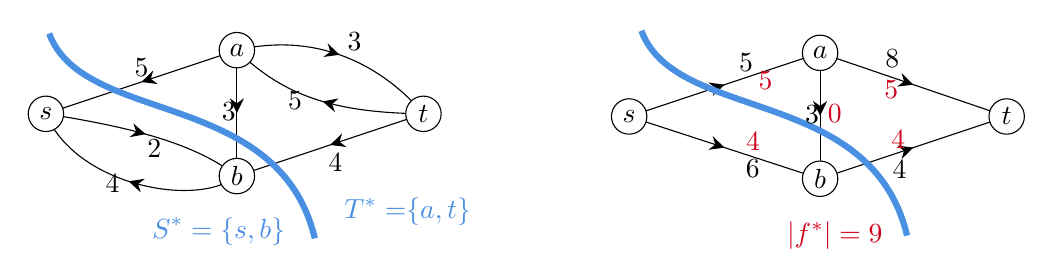
\begin{tikzpicture}[x=0.5pt,y=0.5pt,yscale=-1,xscale=1]
%uncomment if require: \path (0,176); %set diagram left start at 0, and has height of 176

%Straight Lines [id:da09123496908131157] 
\draw    (296,70) -- (161.17,115) ;
\draw [shift={(228.59,92.5)}, rotate = 341.54] [fill={rgb, 255:red, 0; green, 0; blue, 0 }  ][line width=0.08]  [draw opacity=0] (10.72,-5.15) -- (0,0) -- (10.72,5.15) -- (7.12,0) -- cycle    ;
%Straight Lines [id:da19597903283531382] 
\draw [color={rgb, 255:red, 0; green, 0; blue, 0 }  ,draw opacity=1 ]   (161.17,24) -- (23.17,70) ;
\draw [shift={(92.17,47)}, rotate = 341.57] [fill={rgb, 255:red, 0; green, 0; blue, 0 }  ,fill opacity=1 ][line width=0.08]  [draw opacity=0] (10.72,-5.15) -- (0,0) -- (10.72,5.15) -- (7.12,0) -- cycle    ;
%Curve Lines [id:da003967634620389404] 
\draw [color={rgb, 255:red, 0; green, 0; blue, 0 }  ,draw opacity=1 ]   (161.17,24) .. controls (224.88,9.25) and (270.88,40.25) .. (296,70) ;
\draw [shift={(235.42,27.34)}, rotate = 198.02] [fill={rgb, 255:red, 0; green, 0; blue, 0 }  ,fill opacity=1 ][line width=0.08]  [draw opacity=0] (10.72,-5.15) -- (0,0) -- (10.72,5.15) -- (7.12,0) -- cycle    ;
%Curve Lines [id:da9544255371930271] 
\draw    (296,70) .. controls (231.88,69.25) and (194.88,57.25) .. (161.17,24) ;
\draw [shift={(223.07,61.05)}, rotate = 15.31] [fill={rgb, 255:red, 0; green, 0; blue, 0 }  ][line width=0.08]  [draw opacity=0] (10.72,-5.15) -- (0,0) -- (10.72,5.15) -- (7.12,0) -- cycle    ;
%Curve Lines [id:da14332777144371744] 
\draw [color={rgb, 255:red, 0; green, 0; blue, 0 }  ,draw opacity=1 ]   (23.17,70) .. controls (88.88,80.25) and (131.88,92.25) .. (161.17,115) ;
\draw [shift={(95.33,84.71)}, rotate = 195.08] [fill={rgb, 255:red, 0; green, 0; blue, 0 }  ,fill opacity=1 ][line width=0.08]  [draw opacity=0] (10.72,-5.15) -- (0,0) -- (10.72,5.15) -- (7.12,0) -- cycle    ;
%Curve Lines [id:da2638365923485928] 
\draw    (161.17,115) .. controls (132.88,138.25) and (44.88,122.25) .. (23.17,70) ;
\draw [shift={(82.94,118.8)}, rotate = 16.76] [fill={rgb, 255:red, 0; green, 0; blue, 0 }  ][line width=0.08]  [draw opacity=0] (10.72,-5.15) -- (0,0) -- (10.72,5.15) -- (7.12,0) -- cycle    ;
%Straight Lines [id:da47468815088752225] 
\draw [color={rgb, 255:red, 0; green, 0; blue, 0 }  ,draw opacity=1 ]   (161.17,24) -- (161.17,115) ;
\draw [shift={(161.17,69.5)}, rotate = 270] [fill={rgb, 255:red, 0; green, 0; blue, 0 }  ,fill opacity=1 ][line width=0.08]  [draw opacity=0] (10.72,-5.15) -- (0,0) -- (10.72,5.15) -- (7.12,0) -- cycle    ;
%Shape: Ellipse [id:dp954041169370231] 
\draw  [fill={rgb, 255:red, 255; green, 255; blue, 255 }  ,fill opacity=1 ] (10.38,70) .. controls (10.38,62.94) and (16.11,57.21) .. (23.17,57.21) .. controls (30.23,57.21) and (35.96,62.94) .. (35.96,70) .. controls (35.96,77.06) and (30.23,82.79) .. (23.17,82.79) .. controls (16.11,82.79) and (10.38,77.06) .. (10.38,70) -- cycle ;
%Shape: Ellipse [id:dp9013075185816432] 
\draw  [fill={rgb, 255:red, 255; green, 255; blue, 255 }  ,fill opacity=1 ] (283.21,70) .. controls (283.21,62.94) and (288.94,57.21) .. (296,57.21) .. controls (303.06,57.21) and (308.79,62.94) .. (308.79,70) .. controls (308.79,77.06) and (303.06,82.79) .. (296,82.79) .. controls (288.94,82.79) and (283.21,77.06) .. (283.21,70) -- cycle ;
%Shape: Ellipse [id:dp8082050050742036] 
\draw  [fill={rgb, 255:red, 255; green, 255; blue, 255 }  ,fill opacity=1 ] (148.38,24) .. controls (148.38,16.94) and (154.11,11.21) .. (161.17,11.21) .. controls (168.23,11.21) and (173.96,16.94) .. (173.96,24) .. controls (173.96,31.06) and (168.23,36.79) .. (161.17,36.79) .. controls (154.11,36.79) and (148.38,31.06) .. (148.38,24) -- cycle ;
%Shape: Ellipse [id:dp31893054203886095] 
\draw  [fill={rgb, 255:red, 255; green, 255; blue, 255 }  ,fill opacity=1 ] (148.38,115) .. controls (148.38,107.94) and (154.11,102.21) .. (161.17,102.21) .. controls (168.23,102.21) and (173.96,107.94) .. (173.96,115) .. controls (173.96,122.06) and (168.23,127.79) .. (161.17,127.79) .. controls (154.11,127.79) and (148.38,122.06) .. (148.38,115) -- cycle ;

%Straight Lines [id:da18092572046534006] 
\draw    (444.67,71.93) -- (582.67,116.93) ;
\draw [shift={(513.67,94.43)}, rotate = 198.06] [fill={rgb, 255:red, 0; green, 0; blue, 0 }  ][line width=0.08]  [draw opacity=0] (10.72,-5.15) -- (0,0) -- (10.72,5.15) -- (7.12,0) -- cycle    ;
%Straight Lines [id:da026108681541828216] 
\draw    (444.67,71.93) -- (582.67,25.93) ;
\draw [shift={(513.67,48.93)}, rotate = 161.57] [fill={rgb, 255:red, 0; green, 0; blue, 0 }  ][line width=0.08]  [draw opacity=0] (10.72,-5.15) -- (0,0) -- (10.72,5.15) -- (7.12,0) -- cycle    ;
%Straight Lines [id:da4824803197457034] 
\draw    (582.67,25.93) -- (582.67,116.93) ;
\draw [shift={(582.67,71.43)}, rotate = 270] [fill={rgb, 255:red, 0; green, 0; blue, 0 }  ][line width=0.08]  [draw opacity=0] (10.72,-5.15) -- (0,0) -- (10.72,5.15) -- (7.12,0) -- cycle    ;
%Straight Lines [id:da5740743987306038] 
\draw    (582.67,25.93) -- (717.5,71.93) ;
\draw [shift={(650.09,48.93)}, rotate = 198.84] [fill={rgb, 255:red, 0; green, 0; blue, 0 }  ][line width=0.08]  [draw opacity=0] (10.72,-5.15) -- (0,0) -- (10.72,5.15) -- (7.12,0) -- cycle    ;
%Straight Lines [id:da8273834872954168] 
\draw    (582.67,116.93) -- (717.5,71.93) ;
\draw [shift={(650.09,94.43)}, rotate = 161.54] [fill={rgb, 255:red, 0; green, 0; blue, 0 }  ][line width=0.08]  [draw opacity=0] (10.72,-5.15) -- (0,0) -- (10.72,5.15) -- (7.12,0) -- cycle    ;
%Shape: Ellipse [id:dp16280961740768174] 
\draw  [fill={rgb, 255:red, 255; green, 255; blue, 255 }  ,fill opacity=1 ] (431.88,71.93) .. controls (431.88,64.86) and (437.61,59.14) .. (444.67,59.14) .. controls (451.73,59.14) and (457.46,64.86) .. (457.46,71.93) .. controls (457.46,78.99) and (451.73,84.72) .. (444.67,84.72) .. controls (437.61,84.72) and (431.88,78.99) .. (431.88,71.93) -- cycle ;
%Shape: Ellipse [id:dp6732271861876984] 
\draw  [fill={rgb, 255:red, 255; green, 255; blue, 255 }  ,fill opacity=1 ] (704.71,71.93) .. controls (704.71,64.86) and (710.44,59.14) .. (717.5,59.14) .. controls (724.56,59.14) and (730.29,64.86) .. (730.29,71.93) .. controls (730.29,78.99) and (724.56,84.72) .. (717.5,84.72) .. controls (710.44,84.72) and (704.71,78.99) .. (704.71,71.93) -- cycle ;
%Shape: Ellipse [id:dp6687970759594458] 
\draw  [fill={rgb, 255:red, 255; green, 255; blue, 255 }  ,fill opacity=1 ] (569.88,25.93) .. controls (569.88,18.86) and (575.61,13.14) .. (582.67,13.14) .. controls (589.73,13.14) and (595.46,18.86) .. (595.46,25.93) .. controls (595.46,32.99) and (589.73,38.72) .. (582.67,38.72) .. controls (575.61,38.72) and (569.88,32.99) .. (569.88,25.93) -- cycle ;
%Shape: Ellipse [id:dp049465532965687675] 
\draw  [fill={rgb, 255:red, 255; green, 255; blue, 255 }  ,fill opacity=1 ] (569.88,116.93) .. controls (569.88,109.86) and (575.61,104.14) .. (582.67,104.14) .. controls (589.73,104.14) and (595.46,109.86) .. (595.46,116.93) .. controls (595.46,123.99) and (589.73,129.72) .. (582.67,129.72) .. controls (575.61,129.72) and (569.88,123.99) .. (569.88,116.93) -- cycle ;
%Curve Lines [id:da974074023532696] 
\draw [color={rgb, 255:red, 74; green, 144; blue, 226 }  ,draw opacity=1 ][line width=2.25]    (25.5,12) .. controls (50.5,79) and (191.5,51) .. (217.5,160) ;
%Curve Lines [id:da22242750111948206] 
\draw [color={rgb, 255:red, 74; green, 144; blue, 226 }  ,draw opacity=1 ][line width=2.25]    (453.5,10) .. controls (478.5,77) and (619.5,49) .. (645.5,158) ;

% Text Node
\draw (556.88,146.17) node [anchor=north west][inner sep=0.75pt]   [align=left] {$\displaystyle \textcolor[rgb]{0.82,0.01,0.11}{|f^{*} |=9}$};
% Text Node
\draw (196.38,52.14) node [anchor=north west][inner sep=0.75pt]   [align=left] {$\displaystyle 5$};
% Text Node
\draw (64.38,112.14) node [anchor=north west][inner sep=0.75pt]   [align=left] {$\displaystyle 4$};
% Text Node
\draw (85.38,28.14) node [anchor=north west][inner sep=0.75pt]   [align=left] {$\displaystyle 5$};
% Text Node
\draw (161.17,115) node   [align=left] {$\displaystyle b$};
% Text Node
\draw (161.17,24) node   [align=left] {$\displaystyle a$};
% Text Node
\draw (225.59,97) node [anchor=north west][inner sep=0.75pt]   [align=left] {$\displaystyle 4$};
% Text Node
\draw (148.38,60.14) node [anchor=north west][inner sep=0.75pt]   [align=left] {$\displaystyle 3$};
% Text Node
\draw (296,70) node   [align=left] {$\displaystyle t$};
% Text Node
\draw (23.17,70) node   [align=left] {$\displaystyle s$};
% Text Node
\draw (94.67,87) node [anchor=north west][inner sep=0.75pt]   [align=left] {$\displaystyle 2$};
% Text Node
\draw (239.38,9.14) node [anchor=north west][inner sep=0.75pt]   [align=left] {$\displaystyle 3$};
% Text Node
\draw (527.3,81.43) node [anchor=north west][inner sep=0.75pt]  [color={rgb, 255:red, 208; green, 2; blue, 27 }  ,opacity=1 ] [align=left] {$\displaystyle 4$};
% Text Node
\draw (586.3,61.43) node [anchor=north west][inner sep=0.75pt]   [align=left] {$\displaystyle \textcolor[rgb]{0.82,0.01,0.11}{0}$};
% Text Node
\draw (632.3,80.43) node [anchor=north west][inner sep=0.75pt]  [color={rgb, 255:red, 208; green, 2; blue, 27 }  ,opacity=1 ] [align=left] {$\displaystyle 4$};
% Text Node
\draw (627.88,22.06) node [anchor=north west][inner sep=0.75pt]   [align=left] {$\displaystyle 8$};
% Text Node
\draw (522.3,24.43) node [anchor=north west][inner sep=0.75pt]   [align=left] {$\displaystyle 5$};
% Text Node
\draw (527.17,100.93) node [anchor=north west][inner sep=0.75pt]   [align=left] {$\displaystyle 6$};
% Text Node
\draw (444.67,71.93) node   [align=left] {$\displaystyle s$};
% Text Node
\draw (717.5,71.93) node   [align=left] {$\displaystyle t$};
% Text Node
\draw (569.88,62.06) node [anchor=north west][inner sep=0.75pt]   [align=left] {$\displaystyle 3$};
% Text Node
\draw (633.09,101.93) node [anchor=north west][inner sep=0.75pt]   [align=left] {$\displaystyle 4$};
% Text Node
\draw (582.67,25.93) node   [align=left] {$\displaystyle a$};
% Text Node
\draw (582.67,116.93) node   [align=left] {$\displaystyle b$};
% Text Node
\draw (536.3,37.43) node [anchor=north west][inner sep=0.75pt]  [color={rgb, 255:red, 208; green, 2; blue, 27 }  ,opacity=1 ] [align=left] {$\displaystyle 5$};
% Text Node
\draw (627.3,44.43) node [anchor=north west][inner sep=0.75pt]  [color={rgb, 255:red, 208; green, 2; blue, 27 }  ,opacity=1 ] [align=left] {$\displaystyle 5$};
% Text Node
\draw (98,143) node [anchor=north west][inner sep=0.75pt]   [align=left] {$\displaystyle \textcolor[rgb]{0.29,0.56,0.89}{S^{*} =\{s,b\}}$};
% Text Node
\draw (237,129) node [anchor=north west][inner sep=0.75pt]   [align=left] {$\displaystyle \textcolor[rgb]{0.29,0.56,0.89}{T^{*} =}\textcolor[rgb]{0.29,0.56,0.89}{\{}\textcolor[rgb]{0.29,0.56,0.89}{a,t}\textcolor[rgb]{0.29,0.56,0.89}{\}}$};


\end{tikzpicture}

}
\caption{Illustration the proof of the max-flow min-cut theorem.
Left: the residual graph $G_{f^*}$ wrt the flow $f^*$ when FF terminates~(see Figure~4 of Lecture 19).
The cut $(S^*,T^*)$ is constructed by collecting vertices reachable from $s$ in $G_{f^*}$ as $S^*$, and $T^*=V\setminus S^*$.
Right: the same $s$-$t$ cut $(S^*, T^*)$ drawn on the (original) graph $G$, where one can see that for every edge $e\in E(S^*, T^*)$, $f^*(e) = c(e)$,
and for every edge $e\in E(T^*, S^*)$, $f^*(e) = 0$.}
\label{fig:theorem}
\end{figure}


We now show the central result: $|f^*| = c(S^*,T^*)$. Recall the Fact 2 in Lecture
18: the value of any flow, here we focus on $f^*$, can be calculated with any $s$-$t$
cut, and here we will use the particular cut $(S^*,T^*)$.
Specifically, we can write $|f^*| = \sum_{e\in E(S^*, T^*)} f^*(e) - \sum_{e\in E(T^*, S^*)} f^*(e)$.


In fact, we have $f^*(e) = c(e)$ for every $e \in E(S^*,T^*)$. 
See Figure~\ref{fig:theorem}. Why? Suppose conversely that $f^*(e) < c(e)$.
Assume that $e = (u,v)$; the fact that $e = (u,v) \in E(S^*,T^*)$
means that $u \in S^*$ and $v \in T^*$. According to the way the residual graph is constructed, in $G_{f^*}$, there will be
a forward edge $(u,v)$. Consequently, $s$ can reach $v$ in $G_{f^*}$, as $s$ can reach $u$~(because $u\in S^*$) and $u$ can reach 
$v$ following this forward edge. This contradicts to the fact that $v \in T^*$.

Also, we can show that $f^*(e) = 0$ for every $e \in E(T^*,S^*)$. %(Check Figure 4, where $E(T^*,S^*) = \{(a,b)\}$.)
Why? Suppose conversely that $f^*(e)>0$. Assume that $e=(u,v)$; the fact that $e=(u,v) \in E(T^*,S^*)$ means
that $u \in T^*$ and $v\in S^*$. Then in the residual graph $G_{f^*}$, there will be a backward edge 
$(v, u)$. Consequently, $s$ can reach $u$ in $G_{f^*}$, as $s$ can reach $v$~(because $v\in S^*$) and $v$ can reach $u$ following this backward edge. 
This contradicts to the fact that $u \in T^*$.

Combining all above, we have 
$|f^*| = \sum_{e\in E(S^*, T^*)} f^*(e) - \sum_{e\in E(T^*, S^*)} f^*(e)
 = \sum_{e\in E(S^*, T^*)} c(e) - 0 = c(S^*, T^*)$.

This proves that $f^*$ is a maximum-flow and $(S^*,T^*)$ is a minimum $s$-$t$ cut, i.e., the
FF algorithm is optimal, and a minimum-cut can be constructed from the residual
graph. It also completes the connection between the maximum-flow problem and
the minimum-cut problem: for any network, the value of the maximum-flow
always equal to the capacity of the minimum-cut. This is called the max-flow
min-cut theorem.


